\documentclass[12pt,a4paper]{article}
\usepackage[utf8]{inputenc}
\usepackage[T1]{fontenc}
%\usepackage[czech]{babel}
\usepackage{a4wide}
\usepackage{amsmath, amsthm, amsfonts, amssymb, graphicx, url, fancyhdr,multicol,enumerate,mathtools,csquotes,tikz,enumitem,calc,pdfpages}
\newcommand{\norm}[1]{\left\lVert#1\right\rVert}

\newtheorem{theorem}{Theorem}
\newtheorem{lemma}[theorem]{Lemma}
\newtheorem{cor}[theorem]{Corollary}
\newtheorem{prop}[theorem]{Proposition}
\theoremstyle{definition}
\newtheorem{definition}{Definition}[section]

\newcommand{\Cbb}{\mathbb{C}}
\newcommand{\Qbb}{\mathbb{Q}}
\newcommand{\Rbb}{\mathbb{R}}
\newcommand{\Zbb}{\mathbb{Z}}
\newcommand{\Nbb}{\mathbb{N}}
\newcommand{\C}{\mathbb{C}}
\newcommand{\Q}{\mathbb{Q}}
\newcommand{\R}{\mathbb{R}}
\newcommand{\Z}{\mathbb{Z}}
\newcommand{\F}{\mathbb{F}}
%\newcommand{\N}{\mathbb{N}}
\newcommand{\id}{\mathrm{id}}
\newcommand{\im}{\mathrm{im}}
\newcommand{\cok}{\mathrm{coker}}
\newcommand{\Hom}{\mathrm{Hom}}
\newcommand{\Max}{\mathrm{Max}}
\newcommand{\disc}{\mathrm{disc}}
\newcommand{\Gal}{\mathrm{Gal}}
\newcommand{\Tr}{\mathrm{Tr}}
\newcommand{\N}{\mathrm{N}}
\newcommand{\No}{\mathrm{N}_{\Qbb}^K}
\newcommand{\cond}{\text{cond }}
\newcommand{\Ok}{\ensuremath{\mathcal{O}_K}}
\newcommand{\Ol}{\ensuremath{\mathcal{O}_L}}
\newcommand{\Cl}{\ensuremath{\mathcal{C}l}}
\newcommand{\p}{\mathfrak{p}}
\newcommand{\qq}{\mathfrak{q}}
\newcommand{\af}{\mathfrak{a}}
\newcommand{\bb}{\mathfrak{b}}
\newcommand{\rr}{\mathfrak{r}}
\newcommand{\al}{\alpha}
\newcommand{\z}{\zeta}
\newcommand{\zt}{\zeta_{r_3}}
\newcommand{\ev}{\mathrm{ev}}
\newcommand{\uo}{\overline{r_2}}
\newcommand{\vo}{\overline{r_1}}
\newcommand{\Mat}{\ensuremath{\text{Mat}(2,\mathbb{Z})}}
\newcommand{\Char}{\mathrm{char }}
\newcommand{\lcm}{\mathrm{lcm}}
\DeclarePairedDelimiter\abs{\lvert}{\rvert}
\setlist[enumerate,1]{label={\upshape(\roman*)}}

\newcommand\restr[2]{{% we make the whole thing an ordinary symbol
  \left.\kern-\nulldelimiterspace % automatically resize the bar with \right
  #1 % the function
  %\vphantom{\big|} % pretend it's a little taller at normal size
  \right|_{#2} % this is the delimiter
  }}
  
\makeatletter
\newcommand{\DESCRIPTION@original@item}{}
\let\DESCRIPTION@original@item\item
\newcommand*{\DESCRIPTION@envir}{DESCRIPTION}
\newlength{\DESCRIPTION@totalleftmargin}
\newlength{\DESCRIPTION@linewidth}
\newcommand{\DESCRIPTION@makelabel}[1]{\llap{#1}}%
\newcommand{\DESCRIPTION@item}[1][]{%
  \setlength{\@totalleftmargin}%
       {\DESCRIPTION@totalleftmargin+\widthof{\textbf{#1 }}-\leftmargin}%
  \setlength{\linewidth}
       {\DESCRIPTION@linewidth-\widthof{\textbf{#1 }}+\leftmargin}%
  \par\parshape \@ne \@totalleftmargin \linewidth
  \DESCRIPTION@original@item[\textbf{#1}]%
}
\newenvironment{DESCRIPTION}
  {\list{}{\setlength{\labelwidth}{0cm}%
           \let\makelabel\DESCRIPTION@makelabel}%
   \setlength{\DESCRIPTION@totalleftmargin}{\@totalleftmargin}%
   \setlength{\DESCRIPTION@linewidth}{\linewidth}%
   \renewcommand{\item}{\ifx\@currenvir\DESCRIPTION@envir
                           \expandafter\DESCRIPTION@item
                        \else
                           \expandafter\DESCRIPTION@original@item
                        \fi}}
  {\endlist}
\makeatother
  

\begin{document}
%\pagestyle{fancy}                      %Pro větší­ možnosti práce se záhlaví­mi a zápatími
%\fancyhf{}                             %"vvyčištění záhlaví a zápatí"                                         
%\renewcommand{\headheight}{25 pt}                  %
\addtolength{\topmargin}{-30 pt}                   %
\setlength{\headsep}{10 pt}                      %
%\fancyhead[L]{{\emph{M8195/01 Seminář z teorie čísel, podzim 2016, úkol 1}}}  %
%\fancyhead[R]{{\emph{Vladimír Sedláček, učo 408178}}}                 % Nastavení­ pro titulní­ stranu
%\fancyfoot[L]{Školní rok 2009/2010}                %
%\renewcommand{\footrulewidth}{0.8 pt}              %
\renewcommand{\headrulewidth}{1 pt}                %               %

\title{Circular numbers of certain abelian fields}
\author{Vladimír Sedláček}
\date{\today}
\maketitle

Throughout this thesis, we will use the convention that whenever any of the indices $i,j,l,h$ appear on the same line, they are pairwise distinct and moreover $1\leq i,j,l,h\leq 4$, unless stated otherwise. Also for any $n\in \Nbb$, $\zeta_n$ will denote a primitive $n$-th root of unity (WLOG we can take $\zeta_n=e^{2\pi i/n}$). 

\section{Preliminaries}
\begin{definition}
An \textit{abelian field} is a finite Galois extension of $\Q$ with an abelian Galois group. 
\end{definition}

\begin{definition}
The \textit{genus field in the narrow sense} of an abelian field is its maximal extension which is abelian over $\Q$ and unramified at all finite primes. %In this thesis, we will just call it the \textit{genus field}.
\end{definition}

\begin{lemma}\label{genus}
If $K$ is the genus field in the narrow sense of an abelian field $k$ and $P$ is the set of ramified primes of $k$, we have $\Gal(K/\Q)\cong \prod_{p\in P} T_p$, where $T_p$ is the inertia subgroup of $\Gal(K/\Q)$ corresponding to $p$.
\end{lemma}
\begin{proof}
\end{proof}

\begin{theorem}[Kronecker-Weber]
Every abelian field is a subfield of some cyclotomic field.
\end{theorem}
\begin{proof}
\end{proof}

\begin{definition}
Let $k$ be an abelian field. The least number $n\in\mathbb{N}$ such that $k\subseteq \Q(\zeta_n)$ is called the conductor of $k$ and denoted by $\cond k$.
\end{definition}

\begin{definition}
Let $G$ be any group. The (integral) \textit{group ring} $\Z[G]$ is the free $\Z$-module with basis $G$, which is made into a ring, extending linearly the group law on $G$.
\end{definition}

\begin{definition}
An element $\alpha$ of a totally real number field $K$ is called totally positive if for any embedding $\sigma: K\to \R$, we have $\sigma(\alpha)>0$.
\end{definition}

\section{The group of circular numbers}
Let $k$ be a real abelian field, $K$ its the genus field in the narrow sense, $P$ is the set of ramified primes of $k$, $K_p$ is the maximal subfield of $K$ ramified only at $p\in P$. Since $\Gal(K/\Q)$ has a natural action on $K$ (given by evaluating an automorphism on an element), this makes $K$ into a $\Z[\Gal(K/\Q)]$-module. 

\begin{definition}
The group $D(k)$ of circular numbers of $k$ (using Lettl's modification of Sinnott's definition) is given as
$$D:=\big\langle \{-1, \eta_I \big\vert \emptyset \subsetneq I \subseteq P \}\big\rangle_{\Z[\Gal(K/\Q)]},$$
where $\langle \dots \rangle_{\Z[\Gal(K/\Q)]}$ means \enquote{generated as a $\Z[\Gal(K/\Q)]$-submodule of $K$} and $$\eta_I=\text{N}_{\Qbb(\zeta_{\text{cond} \left(\prod_{i\in I}K_i\right)})/\left(\prod_{i\in I}K_i)\right)\cap k}\left(1-\zeta_{\text{cond} \left(\prod_{i\in I}K_i\right)}\right),$$ where $\text{N}$ denotes the norm operator and the product of fields denotes their compositum. The subset of totally positive elements of $D(k)$ will be denoted by $D^+(k)$.
\end{definition}

\begin{definition}
The group $C(k)$ of circular numbers of $k$ is $E(k)\cap D$, where $E(k)$ is the group of units of the ring of algebraic integers of $k$. The subset of totally positive elements of $C(k)$ will be denoted by $C^+(k)$.
\end{definition}

One of the reasons that $C(k)$ is important is the following famous result, due to Sinnott:
\begin{theorem}
The index $[E(k):C(k)]$ is finite.
\end{theorem}
\begin{proof}
\end{proof}

\begin{lemma}\leavevmode
%We have $$C(k)=\big\langle \{-1, \eta_I \big\vert \emptyset \subsetneq I \subseteq P, 1<|I| \}\cup\big\rangle_{\Z[\Gal(K/k)]}$$
\begin{enumerate}%[i)]
\item For $|I|>1$, we have $\eta_I\in E(k)$.
\item For $I=\{p\}$, we have $\eta_I\not\in E(k)$, but $\eta_I^{1-\sigma}\in E(k)$ for any $\sigma\in \Gal(K/\Q)$. % in the inertia subgroup of $\Gal(K/\Q)$ corresponding to $p$.
\end{enumerate}
\end{lemma}
\begin{proof}
\end{proof}

\begin{cor}
We have $$C(k)=\big\langle \{ -1, \eta_I \big\vert I \subseteq P,  |I|\geq 2\} \cup \{\eta_I^{1-\sigma} \big\vert |I|=1, \sigma\in \Gal(K/\Q))\}\big\rangle_{\Z[\Gal(K/\Q]}.$$
\end{cor}

The next result shows that $D^+(k)$ and $C^+(k)$ are free $\Z$-modules.
\begin{lemma}
$D^+(k)$ is a subgroup of $D(k)$ given as $$D^+(k)=\big\langle  \eta_I \big\vert \emptyset \subsetneq I \subseteq P\big\rangle_{\Z[\Gal(K/\Q)]},$$
hence canonically isomorphic to the non-torsion part of $D(k)$. Similarly, $C^+(k)$ is a subgroup of $C(k)$ given as $$C^+(k)=\big\langle \{ \eta_I \big\vert I \subseteq P,  |I|\geq 2\} \cup \{\eta_I^{1-\sigma} \big\vert |I|=1, \sigma\in \Gal(K/\Q))\}\big\rangle_{\Z[\Gal(K/\Q]}.$$
\end{lemma}
\begin{proof}
\end{proof}

\begin{lemma}
The $\Z$-rank of $D^+(k)$ is $[k:\Q]+|P|-1$.
\end{lemma}
\begin{proof}
\end{proof}

\section{Notation and assumptions}
In the remainder of the thesis, we will fix $k$ to be a real abelian field with exactly four ramified primes $p_1,p_2,p_3,p_4$ and we will abbreviate $D(k),D^{+}(k),C(k),C^+(k)$ simply as $D,D^{+},C,C^+$.
\paragraph*{}

 Let $K$ be the genus field in the narrow sense of $k$ and let $G:=\Gal(K/\Q)$. Then by Lemma \ref{genus}, we can identify $G$ with the direct product $T_1\times T_2\times T_3\times T_4$, where $T_i$ is the inertia group corresponding the ramified prime $p_i$. Next, we will define:

\begin{itemize}
\item $H:=\Gal(K/k)$, 
\item $m:=|H|,$
\item the canonical projections $\pi_i:G\to T_i$ ,
\item $a_i:=[T_i:\pi_i(H)]$,
\item $r_i:=|H\cap \ker \pi_i|$,
\item $s_{ij}:=|H\cap \ker (\pi_i\pi_j)|$,
\item $n_i:=\frac{m}{r_i}$,
\item $\eta:=\eta_{\{1234\}}$,
\item $K_i$ as the maximal subfield of $K$ ramified only at $p_i$ (so that $$T_i=\Gal(K/K_jK_lK_h)\cong \Gal(K_i/\Q).)$$
\end{itemize}

We will assume the following:
\begin{itemize}
\item $K\neq k$,
\item $H$ is cyclic, generated by $\tau$,
\item each $T_i$ is cyclic, generated by $\sigma_i$.
\end{itemize}

\section{Auxiliary results}
\begin{lemma}\label{tau}
Without loss of generality, we can assume $\tau=\sigma_1^{a_1}\sigma_2^{a_2}\sigma_3^{a_3}\sigma_4^{a_4}$.
\end{lemma}
\begin{proof}
We know that $a_i=[T_i:\pi_i(H)]$, hence
$\pi_i(\tau)$ generates a subgroup of $T_i$ of index $a_i$. The cyclicity of $T_i$ then implies that $\pi_i(\tau)$ must be the $a_i$-th power of some generator of $T_i$, WLOG $\sigma_i$. The statement now follows, because $\tau$ is determined by its four projections.
\end{proof}

\begin{lemma}\label{comp}
We have $kK_iK_jK_l=K$ and $K_1K_2K_3K_4=K$.
\end{lemma}
\begin{proof}
The extension $K/K_iK_jK_l$ is totally ramified at the prime ideals above $p_h$, so the same must be true for the extension $K/kK_iK_jK_l$. But since the extension $K/k$ is unramified (by the definition of $K$), so is $K/kK_iK_jK_l$. Therefore $[K:kK_iK_jK_l]=1$. The second claim follows from the facts %$\Gal(K_i/\Q)\cong$
$T_i=\Gal(K/K_jK_lK_h)$ and $G=T_1\times T_2\times T_3\times T_4$.
\end{proof}
\begin{center}
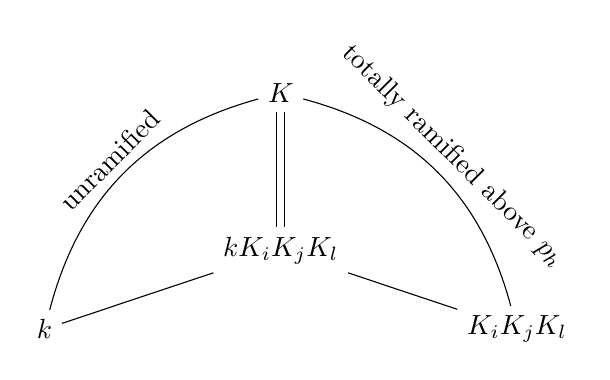
\begin{tikzpicture}
  \node (a) at (0,4)  {$K$};
  \node (b) at (0,2)  {$kK_iK_jK_l$};
  \node (c) at (-3,1)  {$k$};
  \node (d) at (3,1)  {$K_iK_jK_l$};
  \draw[transform canvas={xshift=-1.5pt}] (a) -- (b);
  \draw[transform canvas={xshift=1.5pt}] (b) -- (a);
  \draw   (b) --  (c)
   (b) -- (d);
  \draw[bend left](c) to node [above , sloped]{\text{unramified}}(a);
  \draw[bend right](d) to node [above , sloped]{\text{totally ramified above $p_h$}}(a);
\end{tikzpicture}
\end{center}
%Přidat zvláštní lemma o Galoisových grupách K_iK_jK_l/K_i a podobně kvůli čitelnosti?

\begin{prop}\label{degrees}
We have $a_i=[k\cap K_i:\Q]$, $r_i=[K:kK_i]$, $|T_i|=a_in_i$,  $s_{ij}=[K:kK_iK_j]$. Also $[K_i:k\cap K_i]=n_i$, $[K_iK_j:k\cap K_iK_j]=\frac{m}{s_{ij}}$ and $[K_iK_jK_l:k\cap K_iK_jK_l]=m$.
\end{prop}
\begin{proof}
Since
\begin{equation*}
\begin{split}
\Gal(K/K_i)&=\Gal(K/K_iK_jK_l\cap K_iK_jK_h\cap K_iK_lK_h)\\
&=\Gal(K/K_iK_jK_l)\cdot \Gal(K/K_iK_jK_h)\cdot \Gal(K/K_iK_lK_h)
= T_jT_lT_h
\end{split}
\end{equation*} 
%$$\Gal(K/K_i)\cong \Gal(K/\Q)/\Gal(K_i/\Q)\cong T_1T_2T_3T_4/T_i\cong T_jT_lT_h$$
 and $\Gal(K/k)=H$, it follows that $\Gal(K/k\cap K_i)= T_jT_lT_h\cdot H$. Now consider the short exact sequence %(clearly $\ker \pi_i=T_jT_lT_h$) 
$$0\to H\cap \ker \pi_i\to H \xrightarrow{\restr{\pi_i}{H}} \pi_i(H)\to 0.$$
It follows that $|\pi_i(H)|=\frac{m}{r_i}=n_i$ and $$\pi_i(H)\cong \frac{H}{H\cap \ker \pi_i}=\frac{H}{H\cap T_jT_lT_h}\cong \frac{T_jT_lT_h\cdot H}{T_jT_lT_h}= \frac{\Gal(K/k\cap K_i)}{\Gal(K/K_i)}\cong \Gal(K_i/k\cap K_i).$$
Therefore 
$$[k\cap K_i:\Q]=\frac{|\Gal(K_i/\Q)|}{|\Gal(K_i/k\cap K_i)|}=\frac{|T_i|}{|\pi_i(H)|}=a_i$$
%$$[k\cap K_i:\Q]=\frac{|T_1T_2T_3T_4|}{|T_jT_lT_h\cdot H|}=\frac{|T_1T_2T_3T_4|\cdot |H\cap T_jT_lT_h|}{|T_jT_lT_h|\cdot |H|}=\frac{|T_i|}{|\pi_i(H)|}=a_i.$$
and
$$[K:kK_i]=\frac{|\Gal(K/k)|}{|\Gal(kK_i/k)|}=\frac{|H|}{|\Gal(K_i/k\cap K_i)|}=\frac{m}{|\pi_i(H)|}=r_i.$$
Putting everything together, we obtain $$|T_i|=[K_i:k\cap K_i]\cdot[k\cap K_i:\Q]=a_i|\pi_i(H)|=a_in_i.$$
Next, we also have 
\begin{equation*}
\begin{split}
\Gal(K/K_iK_j)&=\Gal(K/K_iK_jK_l\cap K_iK_jK_h)\\
&=\Gal(K/K_iK_jK_l)\cdot \Gal(K/K_iK_jK_h)= T_lT_h
\end{split}
\end{equation*} 
%$$\Gal(K/K_iK_j)\cong \Gal(K/\Q)/\Gal(K_iK_j/\Q)\cong T_1T_2T_3T_4/T_iT_j\cong T_lT_h,$$
so that $\Gal(K/k\cap K_iK_j)=T_lT_h\cdot H$. Thus we can consider the short exact sequence 
$$0\to H\cap \ker \pi_i\pi_j\to H \xrightarrow{\restr{\pi_i\pi_j}{H}} \pi_i\pi_j(H)\to 0$$
to conclude that $|\pi_i\pi_j(H)|=\frac{m}{s_{ij}}$ and 
\begin{equation*}
\begin{split}
\pi_i\pi_j(H)&\cong \frac{H}{H\cap \ker \pi_i\pi_j}=\frac{H}{H\cap T_lT_h}\cong \frac{T_lT_h\cdot H}{T_lT_h}\\
&\cong \frac{\Gal(K/k\cap K_iK_j)}{\Gal(K/K_iK_j)}\cong \Gal(K_iK_j/k\cap K_iK_j).
\end{split}
\end{equation*}
Then it follows that 
$$[K:kK_iK_j]=\frac{|\Gal(K/k)|}{|\Gal(kK_iK_j/k)|}=\frac{|H|}{|\Gal(K_iK_j/k\cap K_iK_j)|}=\frac{m}{|\pi_i\pi_j(H)|}=s_{ij}.$$
The last part of the statement is a consequence of Lemma \ref{comp}, since we have $$\Gal(K_iK_jK_l/k\cap K_iK_jK_l)\cong \Gal(kK_iK_jK_l/k)=\Gal(K/k)=H.$$
Finally note that in the same way as above, we could show that $$\pi_i\pi_j\pi_l(H)\cong \frac{H}{H\cap T_h}\cong H$$
(since Lemma \ref{comp} implies that $|H\cap T_h|=1$).
%Finally note that in the same way as above, we could show that $$\pi_i\pi_j\pi_l(H)\cong \Gal(K_iK_jK_l/k\cap K_iK_jK_l).$$
\end{proof}
\begin{center}
\begin{tikzpicture}
  \node (a) at (0,4)  {$K$};
  \node (b) at (0,2)  {$kK_i$};
  \node (c) at (-2,0)  {$k$};
  \node (d) at (2,0)  {$K_i$};
  \node (e) at (0,-2)  {$k\cap K_i$};
  \node (f) at (0,-4)  {$\Q$};
  \draw   (a) -- node [left]{$r_i$} (b) -- node [above left]{$n_i$} (c) -- (e) -- node [below right]{$|\pi_i(H)|$} (d) -- node [above right]{$\frac{|T_j\times T_l\times T_h|}{r_i}$} (b)
  (e) -- node [left]{$a_i$} (f);
\end{tikzpicture}
\qquad
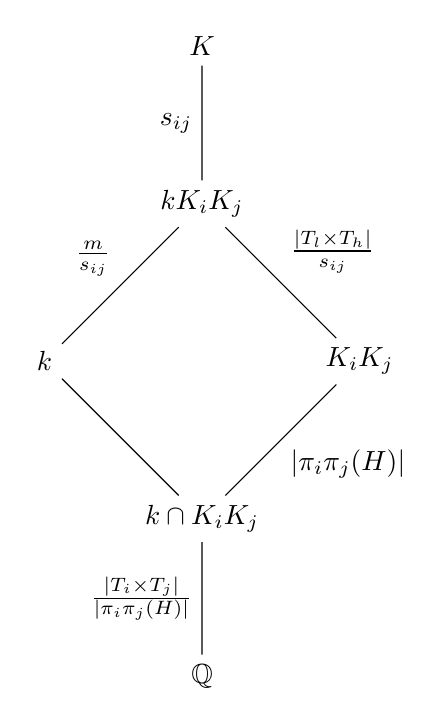
\begin{tikzpicture}
  \node (a) at (0,4)  {$K$};
  \node (b) at (0,2)  {$kK_iK_j$};
  \node (c) at (-2,0)  {$k$};
  \node (d) at (2,0)  {$K_iK_j$};
  \node (e) at (0,-2)  {$k\cap K_iK_j$};
  \node (f) at (0,-4)  {$\Q$};
  \draw   (a) -- node [left]{$s_{ij}$} (b) -- node [above left]{$\frac{m}{s_{ij}}$} (c) -- (e) -- node [below right]{$|\pi_i\pi_j(H)|$} (d) -- node [above right]{$\frac{|T_l\times T_h|}{s_{ij}}$} (b)
  (e) -- node [left]{$\frac{|T_i\times T_j|}{|\pi_i\pi_j(H)|}$} (f);
\end{tikzpicture}
%\vspace{3\baselineskip}
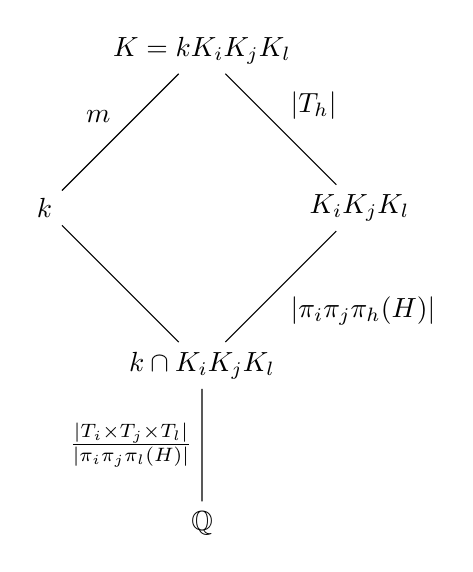
\begin{tikzpicture}
  \node (a) at (0,2)  {$K=kK_iK_jK_l$};
  \node (c) at (-2,0)  {$k$};
  \node (d) at (2,0)  {$K_iK_jK_l$};
  \node (e) at (0,-2)  {$k\cap K_iK_jK_l$};
  \node (f) at (0,-4)  {$\Q$};
  \draw   (a) -- node [above left]{$m$} (c) -- (e) -- node [below right ]{$|\pi_i\pi_j\pi_h(H)|$} (d) -- node [above right]{$|T_h|$} (a)
  (e) -- node [left]{$\frac{|T_i\times T_j\times T_l|}{|\pi_i\pi_j\pi_l(H)|}$} (f);
\end{tikzpicture}
\end{center}

\begin{cor}\label{compcap}
We have $[k\cap K_iK_j:\Q]=a_ia_j\frac{m}{r_ir_j}s_{ij}$, $[k\cap K_iK_jK_l:\Q]=a_ia_ja_l\frac{m^2}{r_ir_jr_l}$ and $[k:\Q]=a_1a_2a_3a_4\frac{m^3}{r_1r_2r_3r_4}$.
\end{cor}
\begin{proof}
This follows from the computations
$$[k\cap K_iK_j:\Q]=\frac{[K_iK_j:\Q]}{[K_iK_j:k\cap K_iK_j]}=\frac{|T_i|\cdot|T_j|}{m/s_{ij}}=a_ia_j\frac{m}{r_ir_j}s_{ij},$$
$$[k\cap K_iK_jK_l:\Q]=\frac{[K_iK_jK_l:\Q]}{[K_iK_jK_l:k\cap K_iK_jK_l]}=\frac{|T_i|\cdot|T_j|\cdot|T_l|}{m}=a_ia_ja_l\frac{m^2}{r_ir_jr_l}$$
and
\begin{equation*}
\begin{split}
[k:\Q]&=\frac{[K:\Q]}{[K:k]}=\frac{|T_1|\cdot|T_2|\cdot|T_3|\cdot|T_4|}{m}=
a_1a_2a_3a_4\frac{m^3}{r_1r_2r_3r_4}.
%[k:\Q]&=[k\cap K_i:\Q]\cdot [k:k\cap K_i]=a_i\cdot [kK_i:K_i]=a_i\frac{[K:K_i]}{[K:kK_i]}\\
%&=a_i\frac{|T_j|\cdot|T_l|\cdot|T_h|}{r_i}=
%a_1a_2a_3a_4\frac{m^3}{r_1r_2r_3r_4}.
\end{split}
\end{equation*}

\end{proof}
\begin{lemma}\label{coprime}
We have 

$$s_{ij}=\gcd(r_i,r_j), \gcd(r_i,r_j,r_l)=1, \lcm\left(n_i,n_j,n_l\right)=m \text{ and } s_{ij}\frac{m}{r_ir_j}=\gcd(n_i,n_j).$$ %(this is also equivalent to $\lcm\left(n_i,n_j,n_l\right)=m$ and to $\gcd(s_{ij},r_l)=1$) 
\end{lemma}
\begin{proof}
It follows from Proposition \ref{degrees} that $s_{ij}\mid r_i, s_{ij}\mid r_j$ and from its proof that $$|\pi_i(H)|=n_i, \quad |\pi_i\pi_j(H)|=\frac{m}{s_{ij}} \text{ and } |\pi_i\pi_j\pi_l(H)|=m.$$ The cyclicity of $H$ then implies
$$\frac{m}{s_{ij}}=|\pi_i\pi_j(H)|=|\langle\pi_i\pi_j(\tau)\rangle|=|\langle\pi_i(\tau)\pi_j(\tau)\rangle|=\lcm\left(n_i,n_j\right),$$
because $\langle\pi_i(\tau)\rangle=\pi_i(H)$ and any power of the product $\pi_i(\tau)\pi_j(\tau)$ is trivial if and only if the same power of both its factors is (since $G$ is the direct product of the $T_i$'s). 
%the elements $\pi_i(H),\pi_j(H)$ have different non-zero coordinates in $G$.
Now for any common divisor $t$ of $r_i,r_j$, we have $$\frac{m}{s_{ij}}= \lcm\left(n_i,n_j\right)=\lcm\left(\frac{m}{r_i},\frac{m}{r_j}\right) \mid \frac{m}{t},$$ which implies $t\mid s_{ij}$. Hence $s_{ij}=\gcd(r_i,r_j)$.

Similarly, we have
$$m=|\pi_i\pi_j\pi_l(H)|=|\langle\pi_i\pi_j\pi_l(\tau)\rangle|=|\langle\pi_i(\tau)\pi_j(\tau)\pi_l(\tau)\rangle|=\lcm(n_i,n_j,n_l),$$
so if $t$ is any common divisor of $r_i,r_j,r_l$, we have $$m=\lcm(n_i,n_j,n_l)=\lcm\left(\frac{m}{r_i},\frac{m}{r_j},\frac{m}{r_l}\right) \mid \frac{m}{t},$$ which implies $t=1$. This implies both $m=\lcm(n_i,n_j,n_l)$ and $\gcd(r_i,r_j,r_l)=1$ (in fact, these are equivalent).

Finally, using the first result, we have $$s_{ij}\frac{m}{r_ir_j}=\frac{m}{r_ir_j/s_{ij}}=\frac{m}{\lcm(r_i,r_j)},$$ which clearly divides both $\frac{m}{r_i}=n_i$ and $\frac{m}{r_j}=n_j$. Moreover, if $t$ is any common divisor of $n_i=\frac{m}{r_i}$ and $n_j=\frac{m}{r_j}$, then both $r_it$ and $r_jt$ divide $m$, hence $t\cdot\lcm(r_i,r_j)=\lcm(r_it,r_jt)\mid m$. Thus $t\mid \frac{m}{\lcm(r_i,r_j)}$ and we are done.
\end{proof}

\begin{prop}\label{gal}
We have 
\begin{equation*}
\begin{split}
\Gal(k/\Qbb)\cong
 \{\restr{\sigma_1^{x_1}\sigma_2^{x_2}\sigma_3^{x_3}\sigma_4^{x_4}}{k};~ & 0\leq x_1<a_1\frac{m}{r_1}, 0\leq x_2<a_2\frac{m}{r_2s_{34}}, \\ & 0\leq x_3<a_3\frac{m}{r_3r_4}s_{34},0\leq x_4<a_4\},
\end{split}
\end{equation*}
where each automorphism of $k$ determines the quadruple $(x_1,x_2,x_3,x_4)$ uniquely.
\end{prop}
\begin{proof}
First note that by Lemma \ref{coprime}, we have $$a_3\frac{m}{r_3r_4}s_{34}=a_3\gcd(n_3,n_4)\in\Nbb$$ and $$a_2\frac{m}{r_2s_{34}}=a_2\lcm(r_3,r_4)\frac{m}{r_2r_3r_4}\in\Nbb$$ (this follows from $r_i\mid m$ and $\gcd(r_2,r_3,r_4)=1$), so the expressions make sense. By Corollary \ref{compcap}, the set on the right hand side has at most $|\Gal(k/\Qbb)|$ elements. Now let $\rho$ be any automorphism of $k$. If we can show that $\rho$ determines the quadruple $(x_1,x_2,x_3,x_4)$ belonging to the set on the right hand side uniquely, it will follow that the cardinalities agree and we will be done. Since $\Gal(k\cap K_4/\Q)$ is a cyclic group of order $a_4$ (by Lemma \ref{degrees}) generated by $\restr{\sigma_4}{k\cap K_4}$ (as a quotient of $\Gal(K_4/\Q)=\langle \restr{\sigma_4}{K_4}\rangle$), there must exist a unique $x_4\in \Z$, $0\leq x_4<a_4$ such that $\rho$ and $\sigma_4^{x_4}$ have the same restrictions to $k\cap K_4$. Therefore $\rho\restr{\sigma_4^{-x_4}}{k}\in \Gal(k/k\cap K_4)$. 

Next, $\Gal(k\cap K_3K_4/k\cap K_4)$ is a cyclic group of order $\frac{[k\cap K_3K_4:\Q]}{[k\cap K_4:\Q]}=a_3\frac{m}{r_3r_4}s_{34}$ (by Corollary \ref{compcap}) generated by $\restr{\sigma_3}{k\cap K_3K_4}$ (as it is isomorphic by restriction to $\Gal((k\cap K_3K_4)K_4 / K_4)$, which is a quotient of $\Gal(K_3K_4/K_4)=\langle \restr{\sigma_3}{K_3K_4}\rangle$), so there must exist a unique $x_3\in \Z$, $0\leq x_3<a_3\frac{m}{r_3r_4}s_{34}$ such that $\rho \restr{\sigma_4^{-x_4}}{k}$ and $\sigma_3^{x_3}$ have the same restriction to $k\cap K_3K_4$. Therefore $\restr{\rho\sigma_3^{-x_3}\sigma_4^{-x_4}}{k}\in \Gal(k/k\cap K_3K_4)$.

Following the pattern, $\Gal(k\cap K_2K_3K_4/k\cap K_3K_4)$ is a cyclic group of order 
$$\frac{[k\cap K_2K_3K_4:\Q]}{[k\cap K_3K_4:\Q]}=a_2\frac{m}{r_2s_{34}}$$ (by Corollary \ref{compcap}) generated by $\restr{\sigma_2}{k\cap K_2K_3K_4}$ (as it is isomorphic by restriction to $\Gal((k\cap K_2K_3K_4)K_3K_4 / K_3K_4)$, which is a quotient of $$\Gal(K_2K_3K_4/K_3K_4)=\langle \restr{\sigma_2}{K_2K_3K_4}\rangle),$$ so there must exist a unique $x_2\in \Z$, $0\leq x_2<a_2\frac{m}{r_2s_{34}}$ such that $\rho\restr{\sigma_3^{-x_3}\sigma_4^{-x_4}}{k}$ and $\sigma_2^{x_2}$ have the same restriction to $k\cap K_2K_3K_4$. Therefore $\restr{\rho\sigma_2^{-x_2}\sigma_3^{-x_3}\sigma_4^{-x_4}}{k}\in \Gal(k/k\cap K_2K_3K_4)$.

Finally, we have $$\Gal(k/k\cap K_2K_3K_4)\cong \Gal(kK_2K_3K_4/K_2K_3K_4)=\Gal(K_1K_2K_3K_4/K_2K_3K_4)=\langle\sigma_1\rangle$$
(using Lemma \ref{comp}), where the isomorphism is given by restriction. Since the order of $\sigma_1$ is $a_1\frac{m}{r_1}$, it follows that there must exist a unique $x_1\in \Z$, $0\leq x_1<a_1\frac{m}{r_1}$ such that $\rho\restr{\sigma_2^{-x_2}\sigma_3^{-x_3}\sigma_4^{-x_4}}{k}$ and $\sigma_1^{x_1}$ have the same restriction to $k$. Thus $\rho=\restr{\sigma_1^{x_1}\sigma_2^{x_2}\sigma_3^{x_3}\sigma_4^{x_4}}{k}$ and the proof is finished.
\begin{center}
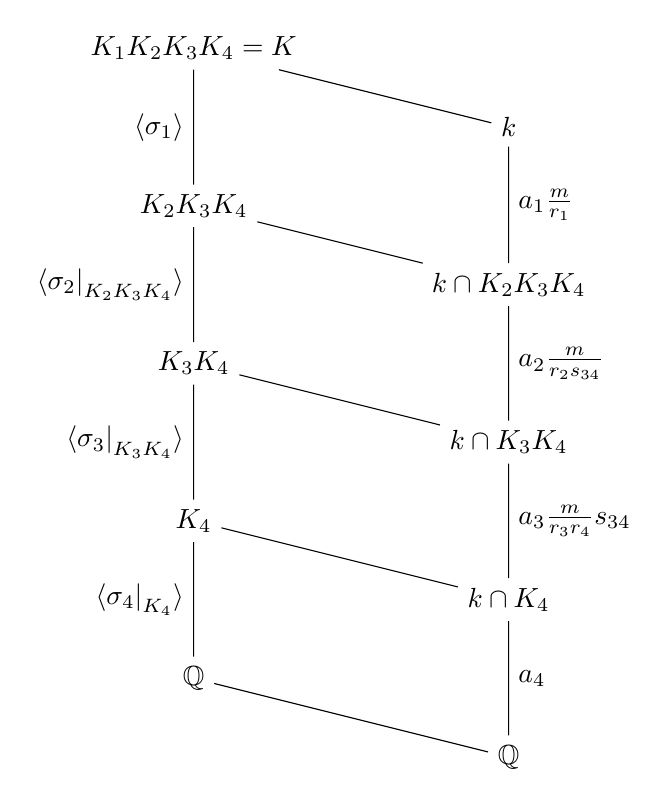
\begin{tikzpicture}
  \node (a) at (0,4)  {$K_1K_2K_3K_4=K$};
  \node (b) at (4,3)  {$k$};
  \node (c) at (0,2)  {$K_2K_3K_4$};
  \node (d) at (4,1)  {$k\cap K_2K_3K_4$};
  \node (e) at (0,0)  {$K_3K_4$};
  \node (f) at (4,-1)  {$k\cap K_3K_4$};
  \node (g) at (0,-2) {$K_4$};
  \node (h) at (4,-3)  {$k\cap K_4$};
  \node (i) at (0,-4) {$\Q$};
  \node (j) at (4,-5)  {$\Q$};
  \draw  (a) -- node [midway,left]{$\langle \sigma_1\rangle$} (c) -- node [midway,left]{$\langle \restr{\sigma_2}{K_2K_3K_4}\rangle$} (e) -- node [midway,left]{$\langle \restr{\sigma_3}{K_3K_4}\rangle$} (g) -- node [midway,left]{$\langle \restr{\sigma_4}{K_4}\rangle$} (i) -- (j) -- node [midway,right]{$a_4$} (h) -- node [midway,right]{$a_3\frac{m}{r_3r_4}s_{34}$} (f) -- node [midway,right]{$a_2\frac{m}{r_2s_{34}}$} (d) -- node [midway,right]{$a_1\frac{m}{r_1}$} (b) -- (a) 
  (c) -- (d)
  (e) -- (f)
  (g) -- (h);
\end{tikzpicture}
\end{center}
\end{proof}

\section{General strategy}

%Recall that $D^+$, the subgroup of totally positive elements of the group $D$ of circular numbers of a real abelian field $k'$ (using Lettl's modification of Sinnott's definition), has one generator $\eta_I$ for each nonempty subset $I\subseteq P$, where $P$ is the set of ramified primes of $k'$. (Since $k'$ is real, $D^+$ is also canonically isomorphic to the non-torsion part of $D$.) 

%More explicitly, if we let $K'_i$ be the largest subfield of $K'$ (the genus field of $k'$ in the narrow sense) ramified only at $p_i$ for any $i\in I$, we have
%$$\eta_I=\text{N}_{\Qbb(\zeta_{\text{cond} \left(\prod_{i\in I}K'_i\right)})/\left(\prod_{i\in I}K'_i)\right)\cap k'}\left(1-\zeta_{\text{cond} \left(\prod_{i\in I}K'_i\right)}\right).$$
%It is well known that $D^+$ is a $\Zbb[G]$-module of $\Zbb$-rank $[k:\Qbb]+|P|-1$. 

%(In our case, we have $k'=k, K'=K, K'_i=K_i, |P|=4$, $\eta:=\eta_{\{1,2,3,4\}}$.)

%The generators of $D^+$ are subject to norm relations (which can be obtained by computing the norm of the generators to a subfield with less ramified primes) and for $|P|\geq 3$, also to the so-called Ennola relations, which are highly nontrivial relations that are not consequences of the norm relations.

%Our goal will be to find a basis of $D^+$ (it can then be easily modified in order to obtain a basis of the group of circular units). Such a basis is known only in a few very special cases though. We would like to construct it for general abelian fields as well, based only on the number of ramified primes.
%\paragraph*{}
Our goal will be to find a basis of $D^+$ (it can then be easily modified in order to obtain a basis of the group of $C^+$). The generators of $D^+$ are subject to norm relations that correspond to the sum of all elements of the respective inertia groups $T_i$. Namely, let $$R_i=\sum_{u=0}^{a_i-1}\sigma_i^u,\, N_i=\sum_{u=0}^{n_i-1}\sigma_i^{ua_i}.$$ 
Then the norm operators from $k$ to a maximal subfield ramified at three primes can be given as $R_iN_i$ (i.e. the sum of all elements of $T_i$). If we denote the congruence corresponding to the canonical projection $\Z[G]\to \Z[G/H]$ by $\equiv$, then we have (using Lemma \ref{tau}) $$N_4\equiv \sum_{u=0}^{n_4-1}\sigma_1^{ua_1}\sigma_2^{ua_2}\sigma_3^{ua_3}.$$ Note that any subgroup of $k^*$ is naturally a $\Z[G/H]$-module, since the action of $H$ on $k$ is trivial.

Moreover, we will denote the congruence corresponding to the composition of canonical projections $$\Z[G]\to \Z[G/H]\to \Z[G/H]/(R_1N_1,R_2N_2,R_3N_3,R_4N_4)$$ by $\sim$, where $(R_1N_1,R_2N_2,R_3N_3,R_4N_4)$ is the ideal generated in $\Z[G/H]$ by the images of the elements $R_iN_i$. When we apply any element of this ideal to the highest generator $\eta$, we will obtain a multiplicative $\Z$-linear combination of circular units belonging to subfields with less ramified primes. We will make use of this extensively.

\begin{lemma}
The fields $$k\cap K_1K_2K_3,k\cap K_1K_2K_4,k\cap K_1K_3K_4,k\cap K_2K_3K_4$$ satisfy the assumptions of [1].
\end{lemma}
\begin{proof}
\end{proof}

To construct a basis of $D^+$, we can take the union of all bases for the fields $$k\cap K_1K_2K_3,k\cap K_1K_2K_4,k\cap K_1K_3K_4,k\cap K_2K_3K_4$$ (we can use the results in [1] to find these) and add in
\begin{equation*}
\begin{split}
N:&=[k:\Q]+3-\sum_{i,j,l}([k\cap K_iK_jK_l:\Q]+2)+\sum_{i,j}([k\cap K_iK_j:\Q]+1)-\sum_{i}[k\cap K_i:\Q]\\&=a_1a_2a_3a_4\frac{m^3}{r_1r_2r_3r_4}-\sum_{i,j,l}a_ia_ja_l\frac{m^2}{r_ir_jr_l}+\sum_{i,j}
a_ia_js_{ij}\frac{m}{r_ir_j}-\sum_{i}a_i+1
\end{split}
\end{equation*}
(by the principle of inclusion and exclusion due to the fact that these bases were constructed \enquote{inductively}) conjugates of $\eta$. 
We cannot guarantee at the moment of all of these conjugates together are not linearly dependent, but of we will show how to obtain all the missing conjugates of $\eta$ using the relations $$R_1N_1\sim 0, R_2N_2\sim 0, R_3N_3\sim 0, R_4\sum_{u=0}^{n_4-1}\sigma_1^{ua_1}\sigma_2^{ua_2}\sigma_3^{ua_3}\sim 0,$$
it will follow that we really have a basis.

We will always refer to the conjugates of $\eta$ by their coordinates $x_1,x_2,x_3,x_4$ according to Proposition \ref{gal}. This allows us to visualise $\Gal(k/\Q)$ geometrically as a discrete (at most) four-dimensional cuboid.
\section{The case $r_1=r_2=r_3=r_4=1$}
\section{The case $r_1=r_2=a_3=r_4=1$}
(Note that in this case we have $s_{34}=1$ and $n_1=n_2=n_4=m$.) %, therefore $$N=a_1a_2a_4\frac{m^3}{r_3}-\sum_{i,j,l}a_ia_ja_l\frac{m^2}{r_ir_jr_l}+\sum_{i,j}+a_ia_js_{ij}\frac{m}{r_ir_j}-\sum_{i}a_i+1.$$
\paragraph*{}
We will add all the conjugates of $\eta$ to our basis except the following cases:
\begin{itemize}
\item $x_1=a_1m-1$ or $x_2=a_2m-1$ or $x_3=n_3-1$,
\item $a_1\leq x_1 < a_1m-1, a_2(m-1)-1 \leq x_2 < a_2m-1, 0\leq x_3 < n_3-1, x_4=0$,
\item $0\leq x_1 < a_1, a_2(m-1) \leq x_2 < a_2m-1, 0\leq x_3 < n_3-1, x_4=0$.
\end{itemize}
These cases are all disjoint, so it's easy to see that the number of conjugates of $\eta$ that we chose is exactly
$$((a_1m-1)a_2(m-2)+(a_1m-1)(a_2-1)+a_1+(a_4-1)(a_1m-1)(a_2m-1))\left(n_3-1\right)=c.$$
\paragraph*{}
First we will recover the cases $0<x_4<a_4$, $x_1=a_1m-1$ or $x_2=a_2m-1$ or $x_3=n_3-1$ using the relations $R_1N_1\sim 0, R_2N_2\sim 0, R_3N_3\sim 0$. From now on, we only need to deal with the cases where $x_4=0$.
\paragraph*{}
Next, we will recover the cases $$x_1=a_1m-1, 0\leq x_2 < a_2(m-1)-1, 0\leq x_3 <n_3-1$$ using the relation $R_1N_1\sim 0$ and subsequently the cases $$0\leq x_1 < a_1m-1, 0\leq x_2 < a_2(m-1)-1, 0\leq x_3 <n_3-1$$ and $$0\leq x_1 < a_1-1, x_2 = a_2(m-1)-1, 0\leq x_3 <n_3-1$$ using the relation $R_3N_3\sim 0$.
\paragraph*{}
Next, we will sequentially recover all the cases $$0\leq x_1 < a_1m-1, a_2(m-1)\leq x_2 < a_2m-1, 0\leq x_3 <n_3-1$$
using the relation $R_4\sum_{u=0}^{m-1}\sigma_1^{a_1u}\sigma_2^{a_2u}\sigma_3^u$. We can do this since any two conjugates of $\eta$ used in this relation differ by at least $a_2$ in their second coordinate. After this, we can recover the cases $$0\leq x_1 < a_1, x_2 = a_2m-1, 0\leq x_3 <n_3-1$$ using the relation $R_2N_2\sim 0$.
\paragraph*{}
Finally, we can use the relation $R_4\sum_{u=0}^{m-1}\sigma_1^{a_1u}\sigma_2^{a_2u}\sigma_3^u$ to recover the cases $$a_1 \leq x_1 <2a_1, x_2 =a_2m-1, 0\leq x_3 <n_3-1$$ and subsequently $R_4\sum_{u=0}^{m-1}\sigma_1^{a_1u}\sigma_2^{a_2u}\sigma_3^u$ to recover the cases $$a_1 \leq x_1 <2a_1, x_2 =a_2(m-1)-1, 0\leq x_3 <n_3-1.$$ By repeating these two steps $(m-2)$ more times, increasing the first coordinate by $a_1$ each time, we will recover all the conjugates.

\section{The case $a_1=a_2=r_3=r_4=1$}
In this case, we have
$$\Gal(k/\Qbb)\cong
 \{\restr{\sigma_1^{x_1}\sigma_2^{x_2}\sigma_3^{x_3}\sigma_4^{x_4}}{k};~  0\leq x_1<n_1, 0\leq x_2<n_2, 0\leq x_3<a_3m,0\leq x_4<a_4\}$$
 and $$N_1\sim 0, N_2\sim 0, R_3N_3 \sim 0, R_4 \sum_{u=0}^{m-1}\sigma_1^u\sigma_2^u\sigma_3^{a_3u} \sim 0.$$

Moreover, by Lemma \ref{coprime}, we have $s_{12}\frac{m}{r_1r_2}=\gcd(n_1,n_2)$, hence
\begin{align*}
N&=a_3a_4\frac{m^3}{r_1r_2}-a_3\frac{m^2}{r_1r_2}-a_4\frac{m^2}{r_1r_2}-a_3a_4\left(\frac{m^2}{r_1}+\frac{m^2}{r_2}\right)+s_{12}\frac{m}{r_1r_2}\\
&+a_3(n_1+n_2)+a_4(n_1+n_2)+a_3a_4m-a_3-a_4-1\\
%&=a_3\left( \frac{m^3}{r_1r_2}-\frac{m^2}{r_1r_2} -\frac{m^2}{r_1}-\frac{m^2}{r_2}+n_1+n_2+m-1\right)+\frac{m^2}{r_1r_2}+n_1+n_2-1+
%\gcd(n_1,n_2)
&=a_3\left(mn_1n_2-n_1n_2 -mn_1-mn_2+n_1+n_2+m-1\right)-n_1n_2+n_1+n_2-1\\
&+(a_4-1)(a_3\left(mn_1n_2 -mn_1-mn_2+m\right)-n_1n_2+n_1+n_2-1)+\gcd(n_1,n_2)-1\\
&=a_3\left(m-1\right)\left(n_1-1\right)\left(n_2-1\right)-\left(n_1-1\right)\left(n_2-1\right)\\
&+(a_4-1)\left(a_3m\left(n_1-1\right)\left(n_2-1\right)-\left(n_1-1\right)\left(n_2-1\right)\right)+\gcd(n_1,n_2)-1\\
&=(n_1-1)(n_2-1)(a_3(m-1)-1)\\
&+(a_4-1)(n_1-1)(n_2-1)(a_3m-1)+\gcd(n_1,n_2)-1.
\end{align*}

We will add the following $N$ conjugates of $\eta$ to our basis:
\begin{itemize}
\item $0\leq x_1<n_1-1, 0\leq x_2<n_2-1, 0\leq x_3<a_3m-1, 0<x_4\leq a_4-1$,
\item $0\leq x_1<n_1-1, 0\leq x_2<n_2-1, a_3<x_3<a_3m, x_4=0$
\item $1\leq x_1<\gcd(n_1,n_2) , x_2=0, x_3=0, x_4=0$.
\end{itemize}

\paragraph*{}
First we will recover the cases $0<x_4<a_4$, $x_1=n_1-1$ or $x_2=n_2-1$ or $x_3=a_3m-1$ using the relations $N_1\sim 0, N_2\sim 0, R_3N_3\sim 0$. From now on, we only need to deal with the cases where $x_4=0$.
\paragraph*{}
Next, we will recover the cases $x_4=0, a_3< x_3<a_3m$, $x_1=n_1-1$ or $x_2=n_2-1$ using the relations $N_1\sim 0, N_2\sim 0$. Now note that the exponents of $\sigma_3$ in $R_4\sum_{u=0}^{m-1}\sigma_1^{u}\sigma_2^{u}\sigma_3^{a_3u}\sim 0$ are pairwise congruent modulo $a_3$. Since for any $1\leq v<a_3$, we can already recover all the conjugates with $x_3\equiv v \pmod{a_3}$ except for one, we can also use the relation $R_4\sum_{u=0}^{m-1}\sigma_1^{u}\sigma_2^{u}\sigma_3^{a_3u}\sim 0$ multiple times to recover the cases $$0\leq x_1<n_1, 0\leq x_2< n_2, 1\leq x_3<a_3, x_4=0$$ as well.
\paragraph*{}
At this moment, we are only missing the conjugates $\eta^{\sigma_1^{x_1}\sigma_2^{x_2}\sigma_3^{a_3}}$ for all $$0\leq x_1<n_1, 0\leq x_2<n_2$$ and $\eta^{\sigma_1^{x_1}\sigma_2^{x_2}}$ for all $$0\leq x_1<n_1, 1\leq x_2<n_2 \text{ and } \gcd(n_1,n_2)\leq x_1<n_1,x_2=0 \text{ and } x_1=x_2=0.$$
We will focus on those of the second kind, because once we have those, we can recover those with $x_3=a_3,x_4=0$ just by using the relation $R_3N_3\sim 0$.

\paragraph*{}
Let $Q'$ be the quotient $\Z[G]$-module $$D^+/\big\langle \{\eta_I \big\vert \emptyset \subsetneq I \subsetneq P \}\big\rangle_{\Z[\Gal(K/\Q)]}$$
and let $Q$ be the quotient $\Z$-module of $Q'$ by the conjugates we have already recovered, i.e.
\begin{align*}
Q:=Q'/\big\langle \{\eta^{\sigma_1^{x_1}\sigma_2^{x_2}\sigma_3^{x_3}\sigma_4^{x_4}}; \quad & 0\leq x_1< n_1, 0\leq x_2<n_2, 0\leq x_3<a_3m,0< x_4<a_4,\\
\text { or }& 0\leq x_1< n_1, 0\leq x_2<n_2, 1\leq x_3<a_3m, x_3\neq a_3, x_4=0,\\
\text { or }& 1\leq x_1<\gcd(n_1,n_2), x_2=x_3=x_4=0 \}\big\rangle_{\Z}.
\end{align*}
We will write $Q$ additively, denoting the class of $\eta$ by $\mu$, hence for any $\rho\in\Gal(k/\Q)$ or $\rho\in\Gal(K/\Q)$, denoting the class of $\eta^{\rho}$ in $Q$ by $\rho\cdot \mu$.
Showing that we have indeed chosen a basis now amounts to showing that $Q$ is trivial. Since $$0=\sigma_1^{x_1}\sigma_2^{x_2}R_3N_3\cdot \mu=\sigma_1^{x_1}\sigma_2^{x_2}\cdot \mu-\sigma_1^{x_1}\sigma_2^{x_2}\sigma_3^{a_3}\cdot \mu$$
for any $x_1,x_2\in\Z$,
this is equivalent with showing that $\sigma_1^{x_1}\sigma_2^{x_2}\cdot \mu=0$ for any $0\leq x_1<n_1, 0\leq x_2<n_2$.

\paragraph*{}
\begin{lemma}\label{diag}
In $Q$, we have $$\sigma_1^{x_1}\sigma_2^{x_2}(1-\sigma_1\sigma_2)\cdot \mu=0$$
for any $x_1,x_2\in\Z$.
\end{lemma}
\begin{proof}
Using the fact that the order of $\sigma_3$ is $a_3m$, we have
\begin{align*}
0&\sim \sigma_1^{x_1}\sigma_2^{x_2}\left(R_3R_4\sum_{u=0}^{m-1}\sigma_1^{u}\sigma_2^{u}\sigma_3^{a_3u}-\sigma_1\sigma_2R_4R_3N_3\right)=\sigma_1^{x_1}\sigma_2^{x_2}R_3R_4\sum_{u=0}^{m-1}\left(\sigma_1^{u}\sigma_2^{u}-\sigma_1\sigma_2\right)\sigma_3^{a_3u}\\
&=\sigma_1^{x_1}\sigma_2^{x_2}(1-\sigma_1\sigma_2)R_3R_4+\sigma_1^{x_1}\sigma_2^{x_2}R_3R_4\sum_{u=2}^{m-1}\left(\sigma_1^{u}\sigma_2^{u}-\sigma_1\sigma_2\right)\sigma_3^{a_3u}\\
&=\sigma_1^{x_1}\sigma_2^{x_2}(1-\sigma_1\sigma_2)+\underbrace{\sigma_1^{x_1}\sigma_2^{x_2}(1-\sigma_1\sigma_2)R_3\sum_{u=1}^{a_4-1}\sigma_4^u}_{\text{contains only terms with } x_4>0}\\
&+\underbrace{\sigma_1^{x_1}\sigma_2^{x_2}(1-\sigma_1\sigma_2)R_4\sum_{u=1}^{a_3-1}\sigma_3^u+\sigma_1^{x_1}\sigma_2^{x_2}R_3R_4\sum_{u=2}^{m-1}\left(\sigma_1^{u}\sigma_2^{u}-\sigma_1\sigma_2\right)\sigma_3^{a_3u}}_{\text{contains only terms with } 1\leq x_3<a_3m \text{ and } x_3\neq a_3}.
\end{align*}
Since all the summands in the expression $$\sigma_1^{x_1}\sigma_2^{x_2}(1-\sigma_1\sigma_2)R_3\sum_{u=1}^{a_4-1}\sigma_4^u
+\sigma_1^{x_1}\sigma_2^{x_2}(1-\sigma_1\sigma_2)R_4\sum_{u=1}^{a_3-1}\sigma_3^u+\sigma_1^{x_1}\sigma_2^{x_2}R_3R_4\sum_{u=2}^{m-1}\left(\sigma_1^{u}\sigma_2^{u}-\sigma_1\sigma_2\right)\sigma_3^{a_3u}$$
have either $x_4>0$ or $ 1\leq x_3<a_3m,  x_3\neq a_3$, the result of their action on $\mu$ becomes trivial in $Q$, which yields the result.
\end{proof}

%Let $X:=\sigma_1^{\gcd(n_1,n_2)-1}\cdot \mu$.

\begin{lemma}
For any $0\leq x_1<n_1, 0\leq x_2<n_2$, we have $$\sigma_1^{x_1}\sigma_2^{x_2}\cdot \mu=\begin{cases}
\mu \quad \text{ if } x_1\equiv x_2 \pmod{\gcd(n_1,n_2)}\\
0 \quad \text{ else}.
\end{cases}$$
\end{lemma}
\begin{proof}
First we will prove that for any $1\leq u<\gcd(n_1,n_2)$ and $0\leq v<\lcm(n_1,n_2)$, we have $$\sigma_1^{u+v}\sigma_2^{v}\cdot \mu=0$$
and $$\sigma_1^{v}\sigma_2^{v}\cdot \mu=\mu.$$
We will do so simultaneously by induction on $v$. For $v=0$, this follows directly from the definitions of $Q$ and $X$. Now suppose that the statements hold for $0\leq v<\lcm(n_1,n_2)-1$. Then Lemma \ref{diag} implies that $$\sigma_1^{u+(v+1)}\sigma_2^{v+1}\cdot \mu=\sigma_1^{u+v}\sigma_2^{v}\cdot \mu=0$$
and $$\sigma_1^{v+1}\sigma_2^{v+1}\cdot \mu=\sigma_1^{v}\sigma_2^{v}\cdot \mu=\mu$$
by the induction hypothesis, so both statements also hold for $v+1$ and we are done with the induction.

\paragraph*{}
Now note that any $0\leq x_1<n_1$, $0\leq x_2<n_2$, we can uniquely write $$x_1-x_2=v\cdot \gcd(n_1,n_2)+u,$$ where $0\leq u<\gcd(n_1,n_2)$ and $0\leq v<n_1\leq \lcm(n_1,n_2)$. Hence $$\sigma_1^{x_1}\sigma_2^{x_2}\cdot\mu=\sigma_1^{v\cdot \gcd(n_1,n_2)+u+x_2}\sigma_2^{x_2}\cdot\mu$$
\end{proof}

\begin{lemma}
We have $\mu=0.$
\end{lemma}
\begin{proof}
\end{proof}
It now follows that $Q$ is trivial, so we are done.

\iffalse
 The conjugates with $x_3=x_4=0$ can be visualized as a discrete rectangle with sides $n_1$ and $n_2$. It is easy to see that such a rectangle can be partitioned into $\gcd(n_1,n_2)$ diagonals, each containing $\lcm(n_1,n_2)$ elements (two conjugates lie in the same diagonal iff their quotient is of the form $\eta^{\sigma_1^v\sigma_2^v}$ for some $v\in\Z$). Now consider the relations $$T:=-\left(\sigma_3^{a_3-1}R_4\sum_{u=0}^{m-1}\sigma_1^{u}\sigma_2^{u}\sigma_3^{a_3u}\right)-\sigma_1^{\frac{m}{r_1}-2}\sigma_2^{\frac{m}{r_2}-2} R_3N_3$$
and
$$S_v:=\sum_{u=0}^{v}\sigma_1^{-u}\sigma_2^{-u}T \text{ for } v\in\Z.$$
Clearly $T\sim 0, S_v\sim 0$ for all $v\in\Z$. Also note that for any $v$, $\eta^{S_v}$ contains no conjugate with $x_3=a_3(m-1)-1$ and contains exactly one conjugate with $x_3=a_3m-1$ that we cannot recover yet minus $\sigma_3^{a_3m-1}$, and these two always lie on the same diagonal. Moreover, any conjugate sharing this diagonal can occur as the one with positive sign for suitable $v\in\Z$. Therefore, since we already have the conjugates $$n_1-(\gcd\left(n_1,n_2\right)-1)\leq x_1\leq n_1-1, \leq x_2=n_2-1, x_3=a_3m-1$$ in our basis, we can recover all the conjugates that share the same diagonal with any (and therefore all) of these.
\paragraph*{}
Now we can recover all the conjugates with $x_3=a_3m-1$ except $\lcm(n_1,n_2)$ of them, which share a diagonal. By using the relation $\sigma_1^{\gcd\left(n_1,n_2\right)-1}\left(S_v-S_w\right)\sim 0$ for suitable $v,w\in\Z$, it is clear that we can generate the difference of any two conjugates lying on this diagonal. Now let $$n_1':=\frac{n_1}{\gcd\left(n_1,n_2\right)}, \quad n_2':=\frac{n_2}{\gcd\left(n_1,n_2\right)}$$ and
note that in each column, there are exactly $n_1'$ conjugates lying on this diagonal, and in each row, there are exactly $n_2'$ conjugates lying on this diagonal. Moreover, we have $$\gcd\left(n_1',n_2'\right)=1$$ by construction,
so there exists an integer $z>0$ such that $$n_2'z\equiv 1\pmod{n_1'}.$$
Using the observation above, we can generate $n_2'z$ differences of conjugates lying on the last diagonal in such a way that we will obtain each of the conjugates in the row $x_1=0$ exactly $z$ times with a negative sign, each of the conjugates in the column $x_2=0$ exactly $\frac{n_2'z-1}{n_1'}$ times with a positive sign and finally one conjugate with a positive sign with $$x_1=n_1-(\gcd\left(n_1,n_2\right)-1)-1,x_2=n_2-1.$$
We can keep this last one and get rid of the rest using the relations $N_1\sim 0$, $N_2\sim 0$. Using this last one, we can generate the rest of its diagonal in the same way as above. Hence we have recovered all the conjugates with $x_3=a_3m-1$. Finally, using the relation $R_3N_3\sim 0$, we can now recover all the conjugates with $x_3=a_3(m-1)-1$ and we are done.
\fi

\section{The case $a_1=a_2=a_3=r_4=1, r_1\neq 1, r_2\neq 1, r_3 \neq 1,\gcd(n_1,n_2,n_3)=\gcd(n_1,n_2)$}

\section{The case $a_1=a_2=a_3=r_4=1, r_1\neq 1, r_2\neq 1, r_3 \neq 1, s_{12}=s_{13}=s_{23}=1,\gcd(n_1,n_2,n_3)=1$}
In this case, we have
\begin{equation*}
\Gal(k/\Qbb)\cong
 \{\restr{\sigma_1^{x_1}\sigma_2^{x_2}\sigma_3^{x_3}\sigma_4^{x_4}}{k};  0\leq x_1<n_1, 0\leq x_2<n_2,  0\leq x_3<n_3,0\leq x_4<a_4\}
\end{equation*}
and $$N_1\sim 0, N_2\sim 0, N_3\sim 0, R_4\sum_{u=0}^{m-1}\sigma_1^u\sigma_2^u\sigma_3^u\sim0.$$
%Note that the condition $\gcd(n_1,n_2,n_3)=1$ is equivalent to $\lcm(r_1,r_2,r_3)=m$, and since we assume that the $r_i$ are pairwise coprime, this is also equivalent to $m=r_1r_2r_3$. Also 
Note that the condition $r_1\neq 1, r_2\neq 1, r_3 \neq 1$ is actually not restrictive, since we have already solved the cases where it is not true. Also $r_1,r_2,r_3$ must be pairwise distinct, otherwise their coprimality would imply that two of them equal $1$. %This means that we can without loss of generality assume that $r_1>r_2>r_3$ (MAYBE NOT NEEDED?). 

\begin{lemma}
Under the assumptions $s_{12}=s_{13}=s_{23}=1,$ the following are equivalent:
\begin{enumerate}%[label={\upshape(\roman*)}]
\item $\gcd(n_1,n_2,n_3)=1$,
\item $\lcm(r_1,r_2,r_3)=m$,
\item $r_1r_2r_3=m$,
\item $n_1=r_2r_3, n_2=r_1r_3, n_3=r_1r_2$,
\item $\frac{n_1n_2n_3}{m}=m$,
\item $\gcd(n_1,n_2)=r_3, \gcd(n_1,n_3)=r_2, \gcd(n_2,n_3)=r_1$.
\end{enumerate}
\end{lemma}
\begin{proof}
\leavevmode
%mbox{}\\
\begin{DESCRIPTION}%[labelindent=0cm]
\item[\enquote{(i) $\Leftrightarrow$ (ii)}:] For any $t\in\Z$, we have
\begin{align*}
t \mid \gcd(n_1,n_2,n_3) &\Leftrightarrow t \mid n_1, t\mid n_2, t\mid n_3 \Leftrightarrow r_1\mid \frac{m}{t}, r_2\mid \frac{m}{t}, r_3\mid \frac{m}{t} \\&\Leftrightarrow \lcm(r_1,r_2,r_3)\mid \frac{m}{t} \Leftrightarrow t \mid \frac{m}{ \lcm(r_1,r_2,r_3)},
\end{align*}
from which it follows that $ \gcd(n_1,n_2,n_3)=\frac{m}{ \lcm(r_1,r_2,r_3)}$.
\item[\enquote{(ii) $\Leftrightarrow$ (iii)}:]   Since $s_{12}=s_{13}=s_{23}=1$, any common multiple of $r_1,r_2,r_3$ is in fact a multiple of $r_1r_2r_3$, hence $\lcm(r_1,r_2,r_3)=r_1r_2r_3$.
\item[\enquote{(iii) $\Leftrightarrow$ (iv)}:] This follows straight from the definition $n_i=\frac{m}{r_i}$.
\item[\enquote{(iii) $\Leftrightarrow$ (v)}:] We have $\frac{n_1n_2n_3}{m}=\frac{m^2}{r_1r_2r_3}$, which equals $m$ iff $\frac{m}{r_1r_2r_3}=1$.
\item[\enquote{(iv) $\Rightarrow$ (vi)}:] For $\{i,j,l\}=\{1,2,3\}$, we have $\gcd(n_i,n_j)=\gcd(r_jr_l,r_ir_l)=r_ls_{ij}=r_l$.
\item[\enquote{(vi) $\Rightarrow$ (i)}:] Since $\gcd(n_1,n_2,n_3)$ must divide $\gcd(n_1,n_2)$, $\gcd(n_1,n_3)$, $\gcd(n_2,n_3)$ and these are pairwise coprime, it must be equal to $1$.
\end{DESCRIPTION}
\end{proof}

Thus $\frac{n_1n_2n_3}{m}=m=r_2n_2=\gcd(n_1,n_3)n_2$ and we have
\begin{align*}
N&=a_4n_1n_2n_3-\frac{n_1n_2n_3}{m}-a_4(n_1n_2+n_1n_3+n_2n_3)-a_4-2+a_4(n_1+n_2+n_3)+\\
&\phantom{am}\gcd(n_1,n_2)+\gcd(n_1,n_3)+\gcd(n_2,n_3)\\
&=(a_4-1)(n_1-1)(n_2-1)(n_3-1)+(n_1-1)(n_2-1)(n_3-2)+\\
&\phantom{am}n_1n_2-(\gcd(n_1,n_3)+1)n_2-(n_1-\gcd(n_1,n_3)-1)+\gcd(n_2,n_3)+\gcd(n_1,n_2)-2\\
&=(a_4-1)(n_1-1)(n_2-1)(n_3-1)+(n_1-1)(n_2-1)(n_3-2)+\\
&\phantom{am}(n_2-1)(n_1-r_2-1)+r_1+r_3-2.
\end{align*}

We will add the following $N$ conjugates of $\eta$ to our basis:
\begin{itemize}
\item $0\leq x_1<n_1-1, 0\leq x_2<n_2-1, 0\leq x_3<n_3-1, 0<x_4\leq a_4-1$,
\item $0\leq x_1<n_1-1, 0\leq x_2<n_2-1, 1< x_3 \leq n_3-1, x_4=0$,
\item $0\leq x_1< n_1-r_2-1, 0\leq x_2<n_2-1, x_3=0, x_4=0$,
\item           $x_1=n_1-r_2-1, 0\leq x_2<r_1+r_3-2, x_3=0, x_4=0$.
\end{itemize}
(Note that $n_1-r_2-1=r_2(r_3-1)-1> 0$ and $r_1+r_3-2>0$ since $r_1,r_2,r_3>1$.)

\paragraph*{}
First we will recover the cases $0<x_4<a_4$, $x_1=n_1-1$ or $x_2=n_2-1$ or $x_3=n_3-1$ using the relations $N_1\sim 0, N_2\sim 0, N_3\sim 0$. From now on, we only need to deal with the cases where $x_4=0$. Next, we will recover the cases $1< x_3 \leq n_3-1$, $x_1=n_1-1$ or $x_2=n_2-1$ (and always $x_4=0$) using the relations $N_1\sim 0, N_2\sim 0$ and the cases $x_3=x_4=0$, $0\leq x_1< n_1-r_2-1$, $x_2=n_2-1$ using the relation $N_2\sim 0$.
\paragraph*{}
At this moment, we are only missing all the cases with $x_3=1,x_4=0$ and some of those with $x_3=x_4=0$. From now on, we will only focus on recovering those with $x_3=x_4=0$, because once we have those, we can recover those with $x_3=1,x_4=0$ just by using the relation $N_3\sim 0$.
\paragraph*{}
From now on, we will write $\uo:=r_2\pmod{r_3}$, $\vo:=r_1\pmod{r_3}$ (so that $\uo,\vo\in\{0,1,\dots,r_3-1\}$) and similarly for other expressions. We will also define $h$ to be the unique integer satisfying $ r_1\cdot h\equiv r_2\pmod{r_3}$ and $h\in\{0,1,\dots,r_3-1\}$ and similarly $h'$ to be the unique integer satisfying $ r_2\cdot h'\equiv r_1\pmod{r_3}$ and $h'\in\{0,1,\dots,r_3-1\}$ (both are well defined, since $\gcd(r_1,r_3)=\gcd(r_2,r_3)=1$). Clearly $h\cdot h'\equiv 1 \pmod{r_3}$.

\paragraph*{}
Let $Q'$ be the quotient $\Z[G]$-module $$D^+/\big\langle \{\eta_I \big\vert \emptyset \subsetneq I \subsetneq P \}\big\rangle_{\Z[\Gal(K/\Q)]}$$
and let $Q$ be the quotient $\Z$-module of $Q'$ by the conjugates we have already recovered, i.e.
\begin{align*}
Q:=Q'/\big\langle \{\eta^{\sigma_1^{x_1}\sigma_2^{x_2}\sigma_3^{x_3}\sigma_4^{x_4}}; \quad & 0\leq x_1< n_1, 0\leq x_2<n_2, 0\leq x_3<n_3,0< x_4<a_4,\\
\text { or }& 0\leq x_1< n_1, 0\leq x_2<n_2, 1< x_3<n_3,x_4=0,\\
\text { or }& 0\leq x_1< n_1-r_2-1, 0\leq x_2<n_2, x_3=x_4=0,\\
\text { or }& x_1= n_1-r_2-1, 0\leq x_2<r_1+r_3-2, x_3=x_4=0 \}\big\rangle_{\Z}.
\end{align*}
We will write $Q$ additively, denoting the class of $\eta$ by $\mu$, hence for any $\rho\in\Gal(k/\Q)$ or $\rho\in Gal(K/Q)$, denoting the class of $\eta^{\rho}$ in $Q$ by $\rho\cdot \mu$.
Showing that we have indeed chosen a basis now amounts to showing that $Q$ is trivial. Since $$0=\sigma_1^{x_1}\sigma_2^{x_2}N_3\cdot \mu=\sigma_1^{x_1}\sigma_2^{x_2}\cdot \mu+\sigma_1^{x_1}\sigma_2^{x_2}\sigma_3\cdot \mu$$
for any $x_1,x_2\in\Z$,
this is equivalent with showing that $\sigma_1^{x_1}\sigma_2^{x_2}\cdot \mu=0$ for each $0\leq x_1<n_1, 0\leq x_2<n_2$.

\paragraph*{}
The conjugates with $x_3=0$ and $x_4=0$ (i.e., those of the form $\eta^{\sigma_1^{x_1}\sigma_2^{x_2}}$) can be visualized as a discrete rectangle with $n_1$ rows and $n_2$ columns. Since for each $x_4$, there are $n_3$ layers of such rectangles in total, the sum $\eta^{R_4\sum_{u=0}^{m-1}\sigma_1^{u}\sigma_2^{u}\sigma_3^{u}}$ must contain $\frac{m}{n_3}=r_3$ conjugates in each of these rectangles. We will now describe the sum of these. 

%Now let $T$ be the sum of the automorphisms contained in  $R_4\sum_{u=0}^{m-1}\sigma_1^{u}\sigma_2^{u}\sigma_3^{u}$ with $x_3=x_4=0$, i.e. 
Let $$T:=\sum_{u=0}^{r_3-1}\sigma_1^{un_3}\sigma_2^{un_3}$$

\begin{lemma}\label{Tdiag}
In $Q$, we have $$\sigma_1^{x_1}\sigma_2^{x_2}(1-\sigma_1\sigma_2)T\cdot \mu=0$$
for any $x_1,x_2\in\Z$.
\end{lemma}
\begin{proof}
Using the fact that every $0\leq w<m$ can be uniquely written as $un_3+v$ with $0\leq u<r_3, 0\leq v<n_3$ together with the fact that the order of $\sigma_3$ is $n_3$, we get 
\begin{align*}
R_4T\sum_{v=0}^{n_3-1}\sigma_1^{v}\sigma_2^{v}\sigma_3^{v}=R_4\sum_{u=0}^{r_3-1}\sigma_1^{un_3}\sigma_2^{un_3}\sigma_3^{un_3}\cdot \sum_{v=0}^{n_3-1}\sigma_1^{v}\sigma_2^{v}\sigma_3^{v}=R_4\sum_{w=0}^{m-1}\sigma_1^{w}\sigma_2^{w}\sigma_3^{w}\sim 0.
\end{align*}
Together with $N_3\sim 0$, this means that 
\begin{align*}
0&\sim \sigma_1^{x_1}\sigma_2^{x_2}\left(R_4T \sum_{v=0}^{n_3-1}\sigma_1^{v}\sigma_2^{v}\sigma_3^{v}-\sigma_1\sigma_2N_3R_4T\right)=\sigma_1^{x_1}\sigma_2^{x_2}R_4T\sum_{v=0}^{n_3-1}\left(\sigma_1^{v}\sigma_2^{v}-\sigma_1\sigma_2\right)\sigma_3^{v}\\
&=\sigma_1^{x_1}\sigma_2^{x_2}(1-\sigma_1\sigma_2)R_4T+\sigma_1^{x_1}\sigma_2^{x_2}R_4T\sum_{v=2}^{n_3-1}\left(\sigma_1^{v}\sigma_2^{v}-\sigma_1\sigma_2\right)\sigma_3^{v}\\
&=\sigma_1^{x_1}\sigma_2^{x_2}(1-\sigma_1\sigma_2)T+\underbrace{\sigma_1^{x_1}\sigma_2^{x_2}(1-\sigma_1\sigma_2)T\sum_{u=1}^{a_4-1}\sigma_4^u+\sigma_1^{x_1}\sigma_2^{x_2}R_4T\sum_{v=2}^{n_3-1}\left(\sigma_1^{v}\sigma_2^{v}-\sigma_1\sigma_2\right)\sigma_3^{v}}_{\text{contains only terms with } x_4>0 \text{ or } x_3>1}.
\end{align*}
Since all the summands in the expression $$\sigma_1^{x_1}\sigma_2^{x_2}(1-\sigma_1\sigma_2)T\sum_{u=1}^{a_4-1}\sigma_4^u+\sigma_1^{x_1}\sigma_2^{x_2}R_4T\sum_{v=2}^{n_3-1}\left(\sigma_1^{v}\sigma_2^{v}-\sigma_1\sigma_2\right)\sigma_3^{v}$$
have either $x_4>0$ or $x_3>1$, the result of their action on $\mu$ becomes trivial in $Q$, which yields the result.
\end{proof}
\paragraph*{}
The rest of the proof will be carried out purely algebraically, but perhaps it is helpful (although not strictly required) to see some of its parts geometrically.

We will decompose our rectangle (of conjugates of $\eta$ having $x_3=x_4=0$) into $r_3\times r_3$ rectangular blocks of height $r_2$ and width $r_1$ in the natural way. In the following, by a big row (resp. big column) we will understand a row of blocks (resp. columns), that is $r_3$ consecutive blocks next to (resp. above) each other. Since $r_2\mid n_3, r_1\mid n_3$ and the conjugates contained in $\eta^T$ are given by $\eta^{\sigma_1^{qn_3}\sigma_2^{qn_3}}$ for $0\leq q \leq r_3-1$, the Chinese remainder theorem implies that $\eta^{\sigma_1^{x_1}\sigma_2^{x_2}T}$ contains exactly one conjugate in every big row (resp. big column) for any $0\leq x_1< n_1, 0\leq x_2< n_2$, and these have the same relative position in each of the respective blocks (determined only by $\vo,\uo,x_1,x_2$). We can be even more precise: the horizontal distance between $\eta^{\sigma_1^{qn_3+x_1}\sigma_2^{qn_3+x_2}}$ and $\eta^ {\sigma_1^{(q+1)n_3+x_1}\sigma_2^{(q+1)n_3+x_2}}$ for $0\leq q \leq r_3-1$ and $0\leq x_1< n_1, 0\leq x_2< n_2$ is exactly $\uo\cdot r_1$, i.e. $\uo$ blocks, and the vertical distance between them is exactly $\vo\cdot r_2$, i.e. $\vo$ blocks (again this follows easily from the Chinese remainder theorem). It follows that the horizontal distance between any two conjugates in $\eta^T$ with a vertical distance of one block is $h$ blocks.

\paragraph*{}
For all $0\leq u\leq n_2$, we will denote $X_u:=\sigma_1^{n_1-2}\sigma_2^{u}\cdot \mu$ and $Y_u:=\sigma_1^{r_2(r_3-1)-1}\sigma_2^u\cdot \mu$. It will be convenient to allow any integers in the indices of the $X$'s and $Y$'s and regard them only modulo $n_2$ (to be more precise, as in the set $\{0,1,\dots,n_2-1\}$). Moreover note that by definition, $Y_u=0$ for $0\leq u< r_1+r_3-2$. 

\begin{lemma}\label{XY}
For any $0\leq x_1<n_1, 0\leq x_2<n_2$, we have
\begin{align*}
\sigma_1^{x_1}\sigma_2^{x_2}\cdot \mu=
\begin{cases}
0   &\text{ if }  x_1<r_2(r_3-1)-1\\
Y_{x_2} \quad &\text{ if } x_1=r_2(r_3-1)-1 \\
X_{\overline{x_2-x_1-2}}  \quad &\text{ if } r_2(r_3-1)\leq x_1<n_1-1 \\
X_{\overline{x_2-x_1-2}}-Y_{x_2-h\cdot r_1} &\text{ if }  x_1=n_1-1.
\end{cases}
\end{align*}
Moreover, we have $X_q=X_{q'}$ for any $q\equiv q'\pmod {r_3}$.
\end{lemma}
\begin{proof}

The first case ($x_1<r_2(r_3-1)-1$) follows directly from the definition of $Q$ and the second case ($x_1=r_2(r_3-1)-1$) directly from the definition of $Y_{x_2}$.

\paragraph*{}
Now for every $0\leq u <n_2$, we will prove by induction with respect to $v=0,1,\dots,r_2-2$ that 
\begin{equation}\label{indX}
\sigma_1^{n_1-2-v}\sigma_2^{u-v}\cdot \mu =X_u.
\end{equation}

The base step $v=0$ is just the definition of $X_u$. Now suppose that $0<v\leq r_2-2$ and the statement holds for $v-1$. Then in the equality
\begin{equation}\label{Teq}
\left(\sigma_1^{n_1-2-v}\sigma_2^{u-v}(1-\sigma_1\sigma_2)\sum_{w=0}^{r_3-1}\sigma_1^{wn_3}\sigma_2^{wn_3}\right)\cdot \mu=0,
\end{equation}
which follows from Lemma \ref{Tdiag}, we claim that all the terms with $w>0$ do not contribute anything to the sum. Indeed, all the exponents of $\sigma_1$ are pairwise congruent modulo $r_2$ (since $r_2\mid n_3$), and since $n_1-r_2\leq n_1-2-v<n_1-2$ and $n_1-r_2+1\leq n_1-1-v<n_1-1$, we have $$\left(\sigma_1^{n_1-2-v}\sigma_2^{u-v}(1-\sigma_1\sigma_2)\sigma_1^{wn_3}\sigma_2^{wn_3}\right)\cdot \mu=0$$ for any $w>0$, because  $r_3$ does not divide $wn_3$ in this case. Hence \eqref{Teq} implies that
$$0=\left(\sigma_1^{n_1-2-v}\sigma_2^{u-v}(1-\sigma_1\sigma_2)\right)\cdot \mu=\sigma_1^{n_1-2-v}\sigma_2^{u-v}\cdot \mu-\underbrace{\sigma_1^{n_1-2-(v-1)}\sigma_2^{u-(v-1)}\cdot \mu}_{=X_u},$$
therefore $\sigma_1^{n_1-2-v}\sigma_2^{u-v}\cdot \mu=X_u$ by the induction hypothesis. This completes the induction, so \eqref{indX} holds. % and proves the third case in the statement of the lemma.

\paragraph*{}
Now for any $0\leq u< n_2$, we will take $v=r_2-1$ in \eqref{Teq}. Again, since all the exponents of $\sigma_1$ are pairwise congruent modulo $r_2$ (since $r_2\mid n_3$) in this sum, the only terms which could be nonzero are those arising from $w=0$ and from $w$ satisfying
$$wn_3+n_1-2-(r_2-1)\equiv n_1-1 \pmod{n_1},$$
which is equivalent to $wn_3\equiv r_2\pmod{n_1}$, which implies $wn_3\equiv r_2\pmod{r_3}$. Together with $wn_3\equiv 0\pmod{r_1}$ and the fact that $\gcd(r_1,r_3)=1$, this means that the only solution to the above congruence is $wn_3\equiv h\cdot r_1\pmod{n_2}$.

Thus we have 
\begin{align*}
0&=\left(\sigma_1^{n_1-r_2-1}\sigma_2^{u-r_2+1}(1-\sigma_1\sigma_2)+\sigma_1^{n_1-1}\sigma_2^{u-r_2+1+h\cdot r_1}(1-\sigma_1\sigma_2)\right)\cdot \mu\\
&=\underbrace{\sigma_1^{n_1-r_2-1}\sigma_2^{u-r_2+1}\cdot\mu}_{=Y_{u-r_2+1}}-\underbrace{\sigma_1^{n_1-r_2}\sigma_2^{u-r_2+2}\cdot\mu}_{=X_u \text{ due to } \eqref{indX}}+\sigma_1^{n_1-1}\sigma_2^{u-r_2+1+h\cdot r_1}\cdot \mu-\underbrace{\sigma_1^{n_1}\sigma_2^{u-r_2+1+h\cdot r_1+1}\cdot \mu}_{=0}.
\end{align*}

Therefore
\begin{equation}\label{indXY}
\sigma_1^{n_1-1}\sigma_2^{u-r_2+1+h\cdot r_1}\cdot \mu = X_u -Y_{u-r_2+1}.
\end{equation}

\paragraph*{}
Finally, for any $0\leq u< n_2$, we will take $v=r_2$ in \eqref{Teq}. Again, since all the exponents of $\sigma_1$ are pairwise congruent modulo $r_2$ in this sum, we only get nonzero terms for $w=0$ and for $w$ satisfying
$$wn_3+n_1-2-r_2\equiv n_1-2 \pmod{n_1},$$ which implies (because we have got the same congruence as above) $wn_3\equiv h\cdot r_1\pmod{n_2}$.

Thus we have 
\begin{align*}
0&=\underbrace{\sigma_1^{n_1-r_2-2}\sigma_2^{u-r_2}\cdot\mu}_{=0}-\underbrace{\sigma_1^{n_1-r_2-1}\sigma_2^{u-r_2+1}\cdot\mu}_{=Y_{u-r_2+1}}
+\underbrace{\sigma_1^{n_1-2}\sigma_2^{u-r_2+h\cdot r_1}\cdot \mu}_{=X_{u-r_2+h\cdot r_1}}-\underbrace{\sigma_1^{n_1-1}\sigma_2^{u-r_2+1+h\cdot r_1}\cdot \mu}_{=X_u-Y_{u-r_2+1} \text{ due to } \eqref{indXY}}.
\end{align*}

Therefore $X_{u -r_2+h\cdot r_1}=X_u$. Note that $$h\cdot r_1-r_2\equiv 0 \pmod{r_3}$$ and $$h\cdot r_1-r_2\equiv -r_2\pmod{r_1}.$$ Since $\gcd(-r_2,r_1)=1$ and $n_2=r_1r_3$, this means that for all $q,q'\in\Z$ satisfying $q\equiv q'\pmod{r_3}$, there is some $w\in\Z$ such that $$q=w(h\cdot r_1-r_2)+q' \pmod{n_2}.$$ But then $$X_q=X_{q+(h\cdot r_1-r_2)}=X_{q+2(h\cdot r_1-r_2)}=\dots=X_{q+w(h\cdot r_1-r_2)}=X_{q'}.$$

\paragraph*{}
Now for any $0\leq u<n_2$, $0\leq v\leq r_2-2$ and $x_1=n_1-2-v,x_2=u-v$, the equality \eqref{indX} implies that $$\sigma_1^{x_1}\sigma_2^{x_2}\cdot \mu=X_u=X_{x_2-x_1-2},$$ since $$x_2-x_1-2=(u-v)-(n_1-2-v)-2=u-n_1\equiv u\pmod {r_3}.$$

Similarly, for any $0\leq u<n_2$, $x_2=u-r_2+1+h\cdot r_1$ and $x_1=n_1-1$, the equality \eqref{indXY} implies that 
$$\sigma_1^{x_1}\sigma_2^{x_2}\cdot \mu=X_u-Y_{u-r_2+1}=X_{x_2-x_1-2}-Y_{x_2-h\cdot r_1},$$ since 
$$x_2-x_1-2=(u-r_2+1+h\cdot r_1)-(n_1-1)-2=u-r_2-h\cdot r_1-n_1\equiv u \pmod{r_3}.$$
This concludes the proof.
\end{proof}

Thanks to Lemma \ref{XY}, from now on we will regard the indices of the $X$'s only modulo $r_3$ (to be more precise, in the set $\{0,1,2,\dots,r_3-1\}$) and drop the bar notation for them. The lemma also implies the equality
\begin{equation}\label{Ycancel}
\sigma_1^{n_1-1}\sigma_2^{x_2}\cdot \mu+\sigma_1^{n_1-r_2-1}\sigma_2^{x_2-h\cdot r_1}\cdot \mu=X_{x_2-1}-Y_{x_2-h\cdot r_1}+Y_{x_2-h\cdot r_1}= X_{x_2-1}
\end{equation}
for any $x_2\in\Z$, which we will use several times. Another simple observation that will come in handy in the proofs of the following lemmas is that the unary operation of adding a fixed integer induces an automorphism of $\Z/r_3$, which we will not mention explicitly anymore.

To show that $Q$ is trivial, it now suffices to show that $X_u=0$ for all $0\leq u< r_3$ and $Y_v=0$ for all $r_1+r_3-2\leq v< n_2$ (knowing already that  $Y_v = 0$ 
for all $0 \le v < r_1 +r_3 - 2$). To achieve this, we will use linear algebra.

%\includepdf[pages=-]{5_export.pdf}
\paragraph*{}
Let $\alpha:= Y_{r_1+r_3-2}+Y_{r_1+r_3-1}+\dots+Y_{n_2-1}\in Q$ and $\beta:=X_0+X_1+\dots+X_{r_3-1}\in Q$.
\begin{lemma}\label{AB}
We have $\alpha=\beta=0$.
\end{lemma}
\begin{proof}
Using the relation $N_2\sim 0$, we have $$0=\sigma_1^{r_2(r_3-1)-1}N_2\cdot \mu =\sum_{x_2=0}^{n_2-1}  \sigma_1^{r_2(r_3-1)-1}\sigma_2^{x_2}\cdot \mu= \sum_{x_2=0}^{n_2-1}Y_{x_2}=\alpha$$ and
\begin{align*}
0&= \sigma_1^{r_2(r_3-1)}N_2\cdot \mu=\sum_{x_2=0}^{n_2-1}  \sigma_1^{r_2(r_3-1)}\sigma_2^{x_2}\cdot \mu=\sum_{x_2=0}^{n_2-1}  X_{x_2-r_2(r_3-1)-2}\\
&=\sum_{x_2=0}^{r_1r_3-1}  X_{x_2+r_2-2}=
\sum_{u=0}^{r_1-1}\sum_{v=0}^{r_3-1} X_{ur_3+v+r_2-2}=r_1\cdot \sum_{v=0}^{r_3-1} X_{v+r_2-2}=r_1\cdot \beta,
\end{align*}
since each $x_2\in\{0,1,\dots,r_1r_3-1\}$ can be uniquely written as $ur_3+v$, where $0\leq u<r_1$, $0\leq v<r_3$.% and the unary operation of adding $r_2-2$ induces an automorphism of $\Z/r_3$.

Similarly, using Lemma \ref{XY} together with the relation $N_1\sim 0$ and the equality \eqref{Ycancel}, %(together with the fact that the operation of subtracting $h$ induces an automorphism of $\Z/r_3$),
we get
\begin{align*}
0&= \sum_{q=0}^{r_3-1} \sigma_2^{qr_1}N_1\cdot \mu =\sum_{q=0}^{r_3-1}\left(\sigma_1^{n_1-1}+\sigma_1^{r_2(r_3-1)-1}\right) \sigma_2^{qr_1}\cdot \mu   
+\sum_{x_1=r_2(r_3-1)}^{n_1-2}\sum_{q=0}^{r_3-1} \sigma_1^{x_1}\sigma_2^{qr_1}\cdot \mu\\
&=\sum_{q=0}^{r_3-1}(\sigma_1^{n_1-1}\sigma_2^{qr_1}+\sigma_1^{r_2(r_3-1)-1}\sigma_2^{(q-h)\cdot r_1})\cdot \mu
+\sum_{x_1=r_2(r_3-1)}^{n_1-2}\sum_{q=0}^{r_3-1} \sigma_1^{x_1}\sigma_2^{qr_1}\cdot \mu\\
&=\sum_{q=0}^{r_3-1}X_{qr_1-1}+\sum_{x_1=r_2(r_3-1)}^{n_1-2}\sum_{q=0}^{r_3-1}X_{qr_1-x_1-2}
= \sum_{x_1=r_2(r_3-1)}^{n_1-1}\sum_{q=0}^{r_3-1}X_{qr_1-x_1-2}
=r_2\cdot \beta,
\end{align*}
since for any $x_1$, all possible remainders modulo $r_3$ occur exactly once as the indices in the sum $\sum_{q=0}^{r_3-1}X_{qr_1-x_1-2}$ (due to the fact that the order of the class of $r_1$ is $r_3$ in $\Z/r_3$, due to their coprimality).
Since $\gcd(r_1,r_2)=1$, this implies $\beta=0$ by Bezout's identity.
\end{proof}

Next, for $0\leq q \leq r_3-3$, we will define $$\Gamma_q:=\sum_{u=0}^{r_3-h'-1}\sum_{v=0}^{\uo-1}X_{q+v-ur_2-1}\in Q.$$

\begin{lemma}
For any $0\leq q \leq r_3-3$, we have $\Gamma_q=0$.
\end{lemma}
\begin{proof}
Using Lemma \ref{XY}, the relation $N_1\sim 0$ and the equality \eqref{Ycancel}, 
we get
\begin{align*}
0&= \sum_{u=0}^{r_3-h'-1} \sigma_2^{q-uhr_1}N_1\cdot \mu\\
&= \sum_{u=0}^{r_3-h'-2}  \underbrace{\left(\sigma_1^{n_1-1}\sigma_2^{q-uh r_1} +\sigma_1^{r_2(r_3-1)-1}\sigma_2^{q-(u+1)h r_1}\right)\cdot \mu}_{=X_{q-uhr_1-1}}\\
&+\underbrace{\sigma_1^{r_2(r_3-1)-1}\sigma_2^q\cdot \mu}_{=Y_q=0}+
\underbrace{\sigma_1^{n_1-1}\sigma_2^{q-(r_3-h'-1)h r_1}\cdot\mu}_{=X_{q-(r_3-h'-1)hr_1-1}-Y_{q+r_1}=X_{q-(r_3-h'-1)hr_1-1}}\\
&+\sum_{x_1=r_2(r_3-1)}^{n_1-2}\sum_{u=0}^{r_3-h'-1} \sigma_1^{x_1}\sigma_2^{q-uh r_1}\cdot \mu,
\end{align*}
where we used the fact that $q\leq r_3-3\leq r_1+r_3-3$ (implying $Y_q=0$) and $$q-(r_3-h'-1)h r_1-hr_1=q-r_1r_3h+r_1hh'\equiv q+r_1\pmod{n_2},$$ since the congruence holds modulo both $r_1$ and $r_3$ (and $\gcd(r_1,r_3)=1$). Also note that $Y_{q+r_1}=0$, since
$$r_1\leq q+r_1\leq r_1+r_3-3,$$
which precisely justifies the bounds on $q$ that we used in the definition of $\Gamma_q$ and also explains why the upper bound in the first sum was chosen to be $r_3-h'-1$.

Continuing with the previous equality and using the congruence $hr_1\equiv r_2\pmod{r_3}$ and Lemma \ref{XY}, we thus have
\begin{align*}
0&= \left(\sum_{u=0}^{r_3-h'-2} X_{q-uhr_1-1}\right)+X_{q-(r_3-h'-1)hr_1-1}+\sum_{x_1=r_2(r_3-1)}^{n_1-2}\sum_{u=0}^{r_3-h'-1} X_{q-uh r_1-x_1-2}\\
&=\sum_{u=0}^{r_3-h'-1} X_{q-ur_2-1}+\sum_{x_1=r_2(r_3-1)}^{n_1-2}\sum_{u=0}^{r_3-h'-1} X_{q-ur_2-x_1-2}\\
&=\sum_{x_1=r_2(r_3-1)}^{n_1-1}\sum_{u=0}^{r_3-h'-1} X_{q-ur_2-x_1-2}\\
&=\sum_{u=0}^{r_3-h'-1} \sum_{v=0}^{r_2-1} X_{q+v-ur_2-1}\\
&=\sum_{u=0}^{r_3-h'-1} \left(\sum_{v=0}^{\overline{r_2}-1} X_{q+v-ur_2-1}+\sum_{v=\overline{r_2}}^{r_2-1} X_{q+v-ur_2-1}\right)\\
&=\sum_{u=0}^{r_3-h'-1} \sum_{v=0}^{\overline{r_2}-1} X_{q+v-ur_2-1}+\sum_{u=0}^{r_3-h'-1}\frac{r_2-\overline{r_2}}{r_3}\sum_{v=\overline{r_2}}^{\overline{r_2}+r_3-1} X_{q+v-ur_2-1}\\
&=\Gamma_q+\sum_{u=0}^{r_3-h'-1}\frac{r_2-\overline{r_2}}{r_3}\cdot \beta=\Gamma_q.
\end{align*}
due to Lemma \ref{AB}.
%since the unary operation of adding $q-ur_2-2$ induces an automorphism of $\Z/r_3$.
\end{proof}

Finally, let $$\Delta:=\sum_{u=0}^{r_3-1}u\cdot\sum_{v=0}^{\uo-1} \sum _{w=0}^{\vo-1} X_{v+w-ur_2-1}\in Q.$$

\begin{lemma}
We have $\Delta=0$.
\end{lemma}
\begin{proof}
Using Lemma \ref{XY}, the relation $N_1\sim 0$ and the equality \eqref{Ycancel},
we get
\begin{align*}
0&= \sum_{u=0}^{r_3-1}u\cdot \sum _{x_2=0}^{r_1-1}\sigma_2^{x_2-uh r_1}N_1\cdot \mu\\
&=\sum_{u=0}^{r_3-1}u\cdot \sum _{x_2=0}^{r_1-1} \left( \sigma_1^{n_1-1}\sigma_2^{x_2-uh r_1}+\sigma_1^{r_2(r_3-1)-1}\sigma_2^{x_2-uh r_1}\right)\cdot \mu\\
&+\sum_{u=0}^{r_3-1}u\cdot \sum_{x_1=r_2(r_3-1)}^{n_1-2}\sum _{x_2=0}^{r_1-1}\sigma_1^{x_1}\sigma_2^{x_2-uh r_1}\cdot \mu\\
&=\sum_{u=0}^{r_3-2} \sum _{x_2=0}^{r_1-1} \left( u\cdot\underbrace{\sigma_1^{n_1-1}\sigma_2^{x_2-uh r_1}\cdot \mu}_{=X_{x_2-uhr_1-1}-Y_{x_2-(u+1)hr_1}}+(u+1)\cdot\underbrace{\sigma_1^{r_2(r_3-1)-1}\sigma_2^{x_2-(u+1)h r_1}\cdot \mu}_{=Y_{x_2-(u+1)h r_1}}\right)+\\
&+\sum_{x_2=0}^{r_1-1}(r_3-1)\cdot \underbrace{\sigma_1^{n_1-1}\sigma_2^{x_2-(r_3-1)h r_1}\cdot \mu}_{=
%X_{x_2-(r_3-1)hr_1-1}-Y_{x_2-hr_1r_3}=
X_{x_2-(r_3-1)hr_1-1}}+\sum_{u=0}^{r_3-1}u\cdot \sum_{x_1=r_2(r_3-1)}^{n_1-2}\sum _{x_2=0}^{r_1-1}\sigma_1^{x_1}\sigma_2^{x_2-uh r_1}\cdot \mu,
\end{align*}

where we used the fact that $$x_2-hr_1r_3\equiv x_2\pmod{n_2}$$  and $0\leq x_2< r_1$, hence $Y_{x_2-hr_1r_3}=0$. Also note that for any $r_1\leq q<n_2$, there exist unique $$u\in\{0,1,\dots,r_3-2\},x_2\in\{0,1,\dots,r_1-1\}$$ such that $$q\equiv x_2-(u+1)hr_1 \pmod{n_2}$$ by the Chinese remainder theorem, since $\gcd(h,r_3)=1$ and for $u=r_3-1$, we would get  $q\equiv r\pmod{n_2}$, where $0\leq r<r_1$.

Continuing with the previous equality and using the congruence $hr_1\equiv r_2\pmod{r_3}$, we thus have

\begin{align*}
0&=\sum_{u=0}^{r_3-2} \sum _{x_2=0}^{r_1-1} u\cdot X_{x_2-ur_2-1}+\sum_{u=0}^{r_3-2} \sum _{x_2=0}^{r_1-1} Y_{x_2-(u+1)hr_1}+\underbrace{\sum_{q=0}^{r_1-1}Y_{q}}_{=0}\\
&+\sum_{x_2=0}^{r_1-1}(r_3-1)\cdot X_{x_2-(r_3-1)r_2-1}+\sum_{u=0}^{r_3-1}u\cdot \sum_{x_1=r_2(r_3-1)}^{n_1-2}\sum _{x_2=0}^{r_1-1}X_{x_2-ur_2-x_1-2}\\
&=\sum_{u=0}^{r_3-1} \sum _{x_2=0}^{r_1-1} u\cdot X_{x_2-ur_2-1}+\sum_{q=r_1}^{n_2-1} Y_{q}+\underbrace{\sum_{q=0}^{r_1-1}Y_{q}}_{=0}\\
&+\sum_{u=0}^{r_3-1}u\cdot \sum_{x_1=r_2(r_3-1)}^{n_1-2}\sum _{x_2=0}^{r_1-1}X_{x_2-ur_2-x_1-2}\\
&=\alpha+\sum_{u=0}^{r_3-1}u\cdot \sum_{x_1=r_2(r_3-1)}^{n_1-1}\sum _{x_2=0}^{r_1-1}X_{x_2-ur_2-x_1-2}\\
%&=\sum_{u=0}^{r_3-1}u\cdot \sum_{x_1=r_2(r_3-1)}^{n_1-1}\sum _{x_2=0}^{r_1-1}X_{x_2-ur_2-x_1-2}\\
&=\sum_{u=0}^{r_3-1}u\cdot \sum_{v=0}^{r_2-1}\sum _{w=0}^{r_1-1}X_{v+w-ur_2-1}\\
&=\sum_{u=0}^{r_3-1}u\cdot \sum_{v=0}^{r_2-1}\left(\sum _{w=0}^{\vo-1}X_{v+w-ur_2-1}+\sum _{w=\vo}^{r_1-1}X_{v+w-ur_2-1}\right)\\
&=\sum_{u=0}^{r_3-1}u\cdot \sum_{v=0}^{r_2-1}\sum _{w=0}^{\vo-1}X_{v+w-ur_2-1}+\sum_{u=0}^{r_3-1}u\cdot \sum_{v=0}^{r_2-1}\frac{r_1-\vo}{r_3}\cdot\sum _{w=\vo}^{\vo + r_3-1}X_{v+w-ur_2-1}\\
&=\sum_{u=0}^{r_3-1}u\cdot \sum _{w=0}^{\vo} \sum_{v=0}^{r_2-1} X_{v+w-ur_2-1}+\sum_{u=0}^{r_3-1}u\cdot \sum_{v=0}^{r_2-1}\frac{r_1-\vo}{r_3}\cdot \beta\\
&=\sum_{u=0}^{r_3-1}u\cdot \sum _{w=0}^{\vo} \sum_{v=0}^{r_1} X_{v+w-ur_2-1}\\
&=\sum_{u=0}^{r_3-1}u\cdot \sum _{w=0}^{\vo}\left( \sum_{v=0}^{\uo-1} X_{v+w-ur_2-1}+\sum_{v=\uo}^{r_2-1} X_{v+w-ur_2-1}\right)\\
&=\sum_{u=0}^{r_3-1}u\cdot \sum _{w=0}^{\vo} \sum_{v=0}^{\uo-1} X_{v+w-ur_2-1}+\sum_{u=0}^{r_3-1}u\cdot \sum _{w=0}^{\vo-1}\frac{r_2-\uo}{r_3}\cdot \sum_{v=\uo}^{\uo+r_3-1} X_{v+w-ur_2-1}\\
&=\Delta+\sum_{u=0}^{r_3-1}u\cdot \sum _{w=0}^{\vo-1}\frac{r_2-\uo}{r_3}\cdot \beta=\Delta.
\end{align*}

\end{proof}

\paragraph*{}
Since $\beta,\Gamma_q$ and $\Delta$ are linear combinations of the $X_u$, they can be written as $\sum_{c=0}^{r_3-1}c_uX_u$, and thus correspond to the $r_3$-tuples of integer coefficients $(c_1,c_2,\dots,c_{r_3})$. Using this correspondence, we will now construct a matrix $M$ of size $r_3\times r_3$ (indexing its dimensions from $0$ to $r_3-1$) as follows:
\begin{itemize}
\item The $0$-th row will correspond to $\beta$ (i.e., it will consist of all 1's).
\item The $q$-th row for $1\leq q\leq r_3-2$ will correspond to $\Gamma_{q-1}$.
\item The $r_3-1$-th row will correspond to $\Delta$.
\end{itemize}

Since the rows of $M$ are coefficients of valid equalities in $Q$, we have $M\cdot X'=0$, where $X=(X_0,X_1,\dots,X_{r_3-1})$ and $'$ denotes transposition. We will show that $M$ is unimodular, i.e. invertible over $\Z$, from which it will follow that $X=0$. To do that, we will study the effect of multiplying $M$ by a character matrix (i.e., basically performing the discrete Fourier transform).
%we will first need to describe $M$ in a better way.

\paragraph*{}
Let $$R(x):=\sum_{q=0}^{r_3-1} x^q\in\Z[x],$$
$$D(x):=\sum_{q=0}^{r_3-1}q\cdot x^q\in \Z[x]$$
and 
$$P(x):=-x^{r_2-1}\cdot \sum_{q=0}^{r_1-1} x^q\in \Z[x].$$

\begin{lemma}\label{RD}
Let $\zeta\neq 1$ be any $r_3$-th root of unity. Then we have $R(\zeta)=0$ and $$D(\zeta)\cdot(\zeta-1)=r_3.$$
\end{lemma}
\begin{proof}
The first assertion is immediate since $R(\zeta)\cdot(\zeta-1)=\zeta^{r_3}-1=0$, but $\zeta\neq 1$. The second follows from the computation
\begin{equation*}
\begin{split}
D(\zeta)\cdot(\zeta-1)&=\sum_{q=1}^{r_3-1} q\cdot \zeta^{q+1}-\sum_{q=1}^{r_3-1} q\cdot \zeta^q=\sum_{q=2}^{r_3} (q-1)\cdot \zeta^{q}-\sum_{q=1}^{r_3-1} q\cdot \zeta^q\\
&=(r_3-1)\zeta^{r_3}+\sum_{q=1}^{r_3-1} (q-1)\cdot \zeta^{q}-\sum_{q=1}^{r_3-1} q\cdot \zeta^q\\
&=r_3-1-\sum_{q=1}^{r_3-1} \zeta^{q}\\
&=r_3- R(\zeta)\\
&=r_3.
\end{split}
\end{equation*}
\end{proof}

Now let $\z$ be any $r_3$-th root of unity and consider the $\Z$-module homomorphism from the free module $\Z[X_0,X_1,\dots,X_{r_3-1}]$ to the cyclotomic field $\Q(\z)$ given by $$\sum_{u=0}^{r_3-1}c_u X_u\mapsto \sum_{u=0}^{r_3-1}c_u \z^u.$$ Since $\beta,\Gamma_q,\Delta \in Z[X_0,X_1,\dots,X_{r_3-1}]$ for $0\leq q\leq r_3-3$, we can apply this homomorphism to them, and we will denote its respective values by $\beta(\z),\Gamma_q(\z),\Delta(\z)\in\Q(\z)$. Note that since $\z^{r_3}=1$, these values depend on the indices of $X_u$ only modulo $r_3$, so it doesn't matter whether we regard them as in the set $\{0,1,\dots,r_3-1\}$ or just as integers. This will allow us to use the original definitions of $\beta,\Gamma_q,\Delta$ for their computation quite easily.

\begin{lemma}\label{argeo}
For any $a,b\in\Nbb$ and $x\in\C$, we have the equality
$$(x^a-1)\cdot\sum_{u=1}^{b}u\cdot x^{ua}=(b+1)x^{a(b+1)}-\sum_{u=0}^b x^{a(b+1)}.$$
\end{lemma}
\begin{proof}
Let $y=x^a$. If $y=0$, both sides are equal to $0$. So suppose $y\neq 0$, then we have 
\begin{align*}
\sum_{u=1}^{b}u\cdot x^{ua}&=\sum_{u=0}^{b}u\cdot y^{u}=y\cdot \sum_{u=0}^{b}u\cdot y^{u-1}=y\cdot \sum_{u=0}^{b}\frac{\partial}{\partial y} y^u=y\cdot \frac{\partial}{\partial y}\sum_{u=0}^{b} y^u\\
&=y\cdot \frac{\partial}{\partial y} \left(\frac{y^{b+1}-1}{y-1}\right)=y\cdot \left(\frac{(b+1)y^{b}(y-1)-(y^{b+1}-1)}{(y-1)^2}\right)\\
&=y\cdot \left(\frac{(b+1)y^{b}-\sum_{u=0}^b y^u}{y-1}\right)=\frac{(b+1)y^{b+1}-\sum_{u=0}^b y^{u+1}}{y-1}\\
&=\frac{(b+1)x^{a(b+1)}-\sum_{u=0}^b x^{a(b+1)}}{x^a-1}.
\end{align*}
By multiplying this equality by $x^a-1$, we obtain the result.
\end{proof}

\begin{lemma}
Let $\zeta\neq 1$ be any $r_3$-th root of unity. Then for all $0\leq q<r_3-3$, we have $$\beta(\z)=0,$$ $$\Gamma_q(\zeta)=\zeta^{q}\cdot P(\zeta)$$ and $$\Delta(\zeta)=D(\zeta)\cdot P(\zeta).$$
\end{lemma}
\begin{proof}
Note that $\z^{-r_2}\neq 1$, since $\gcd(r_3,-r_2)=1$ and $\z\neq1$.

From the definitions and Lemma \ref{RD}, we directly get $\beta(\z)=R(\z)=0$. For the second assertion, we have
\begin{equation*}\label{Gamma}
\begin{split}
\Gamma_q(\zeta)&=\sum_{u=0}^{r_3-h'-1}\sum_{v=0}^{\uo-1}\z^{q+v-ur_2-1}\\
&=\z^{q-1}\cdot\sum_{v=0}^{\uo-1}\z^{v}\sum_{u=0}^{r_3-h'-1}\z^{-ur_2}\\
&=\z^{q-1}\cdot(1+\zeta+\dots+\zeta^{\uo-1})(1+\zeta^{-r_2}+\zeta^{-2r_2}+\dots+\zeta^{-(r_3-h'-1)r_2})\\
&=\zeta^{q-1}\cdot\frac{\zeta^{\uo}-1}{\zeta-1}\cdot \frac{\zeta^{-(r_3-h')r_2}-1}{\zeta^{-r_2}-1}\\
&=\zeta^{q-1}\cdot\frac{\zeta^{r_2}-1}{\zeta^{-r_2}-1}\cdot \frac{\zeta^{r_1}-1}{\zeta-1}\\
&=-\zeta^{q}\cdot \zeta^{r_2-1}\cdot (1+\zeta+\zeta^2+\dots+\zeta^{r_1-1})\\
&=\zeta^{q}\cdot P(\zeta).
\end{split}
\end{equation*}

Similarly, using Lemma \ref{argeo} with $a=\overline{-r_2}$ and $b=r_3-1$, we can see that

\begin{equation*}\label{Delta}
\begin{split}
\Delta(\zeta)&=
\sum_{u=0}^{r_3-1}u\cdot\sum_{v=0}^{\uo-1} \sum _{w=0}^{\vo-1} \z^{v+w-ur_2-1}\\
&=\z^{-1}\cdot\sum_{v=0}^{\uo-1}\z^v \sum _{w=0}^{\vo-1} \z^{w}\sum_{u=0}^{r_3-1}u\cdot\z^{-ur_2}\\
&=\z^{-1}(1+\z+\!\dots\!+\z^{\uo-1})(1\!+\z+\!\dots\!+\z^{\vo-1})(\z^{-r_2}+2\z^{-2r_2}+\!\dots\!+(r_3-1)\z^{-(r_3-1)r_2})\\
&=\z^{-1} \cdot \frac{\zeta^{\uo}-1}{\zeta-1}\cdot \frac{\zeta^{\vo}-1}{\zeta-1}\cdot \frac{r_3\z^{\overline{-r_2}r_3}-\sum_{u=0}^{r_3-1}\z^{\overline{-r_2}(u+1)}}{\z^{\overline{-r_2}}-1}
\\
&=\z^{-1} \cdot \frac{\zeta^{\uo}-1}{\zeta-1}\cdot \frac{\zeta^{\vo}-1}{\zeta-1}\cdot \frac{r_3(\z^{r_3})^{r_2}-\zeta^{-r_2}\cdot R(\zeta^{-r_2})}{\z^{-r_2}-1}
\\
&=\z^{-1}\cdot\frac{\zeta^{r_2}-1}{\zeta-1}\cdot \frac{\zeta^{r_1}-1}{\zeta-1} \cdot \frac{r_3}{\zeta^{-r_2}-1}\\
&=\z^{-1}\cdot\frac{r_3}{\zeta-1}\cdot \frac{\zeta^{r_2}-1}{\zeta^{-r_2}-1}\cdot \frac{\zeta^{r_1}-1}{\zeta-1}\\
&=-D(\zeta)\cdot \zeta^{r_2-1}\cdot (1+\zeta+\zeta^2+\dots+\zeta^{r_1-1})\\
&=D(\zeta)\cdot P(\zeta).
\end{split}
\end{equation*}
\end{proof}

\begin{theorem}
$M$ is unimodular, hence $X=0$.
\end{theorem}
\begin{proof}
Let $\zt$ be a primitive $r_3$-th root of unity and let $C$ be the corresponding $r_3\times r_3$ character matrix, i.e. $C=(\zt^{r\cdot c})_{0\leq r,c<r_3}$. We will use the two previous lemmas together with the fact that multiplying a column of successive powers of $\zt$ by a row of $M$ from the left corresponds to evaluating the polynomial obtained from this row at $\zt$. %After reindexing the dimensions of $M$ from $0$ to $r_3-1$, we have
Hence we have $M\cdot C=C'$, where $C'_{0,0}=R(1)=r_3$ and the $c-th$ column of $C'$ is
$$
\begin{pmatrix}
R(\zt^c)\\ 
P(\zt^c) \\ 
\zt^c \cdot P(\zt^c) \\ 
(\zt^{c})^2 \cdot P(\zt^c) \\ 
\vdots\\ 
(\zt^{c})^{r_3-3} \cdot P(\zt^c) \\ 
D(\zt^c) \cdot P(\zt^c)
\end{pmatrix}
=
\begin{pmatrix}
0\\ 
P(\zt^c) \\ 
\zt^c \cdot P(\zt^c) \\ 
\zt^{2c} \cdot P(\zt^c) \\ 
\vdots\\ 
\zt^{(r_3-3)c} \cdot P(\zt^c) \\ 
D(\zt^c) \cdot P(\zt^c)
\end{pmatrix}
$$
for any $0<c<r_3$ (we don't need to specify the rest of the $0$-th column, since it doesn't influence the determinant of $C'$). Thus by taking out $P(\zt^c)$ from each of these columns, we get (using that multiplication by $r_1$ is an automorphism of $\Z/r_3$, since $\gcd(r_1,r_3)=1$)
$$|\det C'|=|\det C''|\cdot\abs*{\prod_{0<c<r_3}P(\zt^c)}=|\det C''|\cdot\abs*{\prod_{0<c<r_3}-\zt^{c(r_2-1)}}\cdot\abs*{\prod_{0<c<r_3}\frac{\zt^{cr_1}-1}{\zt^c-1}}=|\det C''|,$$
where
$$C''=
\begin{pmatrix}
r_3& 0& \dots & 0 & \dots & 0\\ 
*& 1& \dots & 1 & \dots & 1\\ 
*& \zt& \dots & \zt^c & \dots & \zt^{r_3-1}\\ 
*& \zt^2& \dots & \zt^{2c} & \dots & \zt^{2(r_3-1)}\\ 
\vdots& \vdots&\ddots  & \vdots & \ddots & \vdots\\ 
*& \zt^{r_3-3}& \dots & \zt^{(r_3-3)c} & \dots & \zt^{(r_3-3)(r_3-1)}\\ 
*& D(\zt)& \dots & D(\zt^c) & \dots & D(\zt^{r_3-1})\\ 
\end{pmatrix}.
$$
On the other hand, if we take the matrix $C$, add all of its rows to the last one (thus creating $\begin{pmatrix}
r_3 & 0 & 0& \dots &0
\end{pmatrix}$
there) and then add a suitable linear combination of rows $0,1,\dots, r_3-3$ to the $r_3-2$-th row multiplied by $-1$ using the equality
$$-\zt^{(r_3-2)c}+(r_3-1)\cdot\underbrace{\sum_{u=0}^{r_3-1}\zt^{uc}}_{=0}+\sum_{u=0}^{r_3-3}(u-r_3+1)\cdot\zt^{uc}=\sum_{u=0}^{r_3-1}u\cdot\zt^{uc},$$
so that the $r_3-2$-th row will become
$$\begin{pmatrix}
*& D(\zt)& \dots & D(\zt^c) & \dots & D(\zt^{r_3-1})
\end{pmatrix},$$
we will obtain a matrix with the same determinant as $C''$ (up to a sign). Since the elementary row operations preserve the determinant up to a sign, it follows that
$$|\det C|=|\det C''|=|\det C'|=|\det M|\cdot |\det C|.$$ 
Now, $C$ can be seen as a special type of a Vandermonde matrix, so we have $$\det C=\prod_{0\leq r<c<r_3}(\zt^r-\zt^c)\neq 0$$
(in fact it is well known that this equals $\pm \sqrt{r_3^{r_3}}$), which implies that %$|\det M'|=1$, hence%
 $|\det M|=1$, as needed.
\end{proof}

\begin{cor}
We have $Y_q=0$ for all $r_1+r_3-2\leq q\leq n_2-1$.
\end{cor}
\begin{proof}
By the Chinese remainder theorem, it suffices to show by induction with respect to $u=0,1,\dots,r_3-1$ that for any $0\leq v<r_1$, we have $Y_{v-uhr_1}=0.$ The base case $u=0$ follows directly from the definition of $Y_u$. Now suppose the statement is true for $0\leq u<r_3-1$. Then using $N_1\sim 0$ and Lemma \ref{XY}, we get
\begin{align*}
0&=\sigma_2^{v-uhr_1} N_1 \cdot \mu=\sum_{x_1=r_2(r_3-1)-1}^{n_1-1}\sigma_1^{x_1}\sigma_2^{v-uhr_1}\cdot\mu\\
&=\underbrace{Y_{v-uhr_1}}_{=0}-Y_{v-uhr_1-hr_1}+\sum_{x_1=r_2(r_3-1)}^{n_1-1}\underbrace {X_{v-uhr_1-x_1-2}}_{=0}=-Y_{v-(u+1)hr_1}
\end{align*}
by the induction hypothesis and the fact that $X=0$. This completes the induction.
\end{proof}

It now follows that $Q$ is trivial, so we are done.
\section{The module of relations}
\section{Construction of suitable abelian fields}
Let $m,a_1,a_2,a_3,a_4,r_1,r_2,r_3,r_4$ be positive integers such that 
$$m>1, r_i\mid m, \gcd(r_i,r_j,r_l)=1.$$
We will construct an infinite family of fields $k$ that satisfy all of our assumptions such that these integers correspond to the parameters in our problem of the same name (again we will denote $n_i=\frac{m}{r_i}$).

First, we will fix distinct primes $p_1,p_2,p_3,p_4$ such that $p_i\equiv 1\pmod{ 2a_in_i}$ (by Dirichlet's theorem on primes in arithmetic progressions, there are infinitely many ways of doing this). Then there exist even Dirichlet characters $\chi_i$ of conductors $p_i$ and orders $a_in_i$ (namely, these can be given as $\chi_i:=\chi^{\frac{p_i-1}{a_in_i}}$, where $\chi$ is any generator of the cyclic group $\widehat{(\Z/p_i\Z)^\times}$ (note that $p_i>2$)).

Now let $K_i$ be the field associated to $\langle \chi_i\rangle$. Then $K_i$ is real (because $\chi_i$ is even) and $\Gal(K_i/\Q)$ is cyclic of order $a_in_i$, say $\Gal(K_i/\Q)=\langle \sigma_i\rangle$. Moreover, since the conductors $p_i$ are coprime, the group $\langle \chi_1,\chi_2,\chi_3,\chi_4\rangle$ corresponds to the compositum field $K=K_1K_2K_3K_4$. By the theory of Dirichlet characters, $K$ is ramified exactly at primes $p_i$ (with inertia subgroups isomorphic to $\Gal(K_i/\Q)$) and $$\Gal(K/\Q)=\Gal(K_1/\Q)\Gal(K_2/\Q)\Gal(K_3/\Q)\Gal(K_4/\Q)=\langle\sigma_1,\sigma_2,\sigma_3,\sigma_4\rangle,$$
so that $[K:\Q]=a_1a_2a_3a_4\frac{m^4}{r_1r_2r_3r_4}$. Now let $\tau:=\sigma_1^{a_1}\sigma_2^{a_2}\sigma_3^{a_3}\sigma_4^{a_4}$ and let $k$ be the subfield of $K$ fixed by $\tau$. Since $k$ is a subfield of a compositum of real fields, it must also be real. In order to reach our goal, we now only need to prove the following theorem (it is not hard to see that we could have used the results from Lemma \ref{comp} and Proposition \ref{degrees} as definitions instead).

\begin{theorem}
In the above notation, we have $[K:k]=m$, $[K:kK_i]=r_i$, $[k\cap K_i:\Q]=a_i$ and $kK_iK_jK_l=K$ (i.e. $K$ is the genus field in the narrow sense of $k$).
\end{theorem}
\begin{proof}
Using Lemma \ref{coprime} several times, we can compute
$$[K:k]=|\langle\tau\rangle|=\lcm\left(n_i,n_j,n_l\right)=m,$$
$$[K:kK_i]=|\langle\tau\rangle\cap \langle\sigma_j\sigma_l\sigma_h\rangle|=|\langle\tau^{a_in_i}\rangle|=r_i,$$
$$[k\cap K_i:/\Q]=[\langle\sigma_1,\sigma_2,\sigma_3,\sigma_4\rangle:\langle\tau,\sigma_j,\sigma_l,\sigma_h\rangle]=[\langle\sigma_1,\sigma_2,\sigma_3,\sigma_4\rangle:\langle\sigma_i^{a_i},\sigma_j,\sigma_l,\sigma_h\rangle]=a_i$$
and
$$[K:kK_iK_jK_l]=|\langle\tau\rangle\cap \langle\sigma_h\rangle|=|\langle\tau^{\lcm\left(n_i,n_j,n_l\right)}\rangle|=|\langle\tau^m\rangle|=1.$$
\end{proof}
\end{document}
